%----------------------------------------------------------------------------------------
%   PACKAGES AND DOCUMENT CONFIGURATIONS
%----------------------------------------------------------------------------------------

\documentclass[captions=tableheading,a4paper,11pt,numbers=noenddot,headsepline,titlepage,twoside,openright,DIV=14,BCOR=8mm,parskip=half]{scrbook}
\PassOptionsToPackage{obeyspaces}{url}
\usepackage[backend=biber,
            autocite=plain,
            sorting=none,
            url=false
            ]{biblatex}
\usepackage[T1]{fontenc}
\usepackage[shortlabels]{enumitem}
\usepackage{siunitx}
\usepackage{array}
\usepackage{ccicons}
\usepackage{booktabs}
\usepackage{xspace}
\usepackage{xcolor}
\usepackage{minted}
\usemintedstyle{tango}
\usepackage{a4wide}
\usepackage{listings}
\usepackage{graphicx}
\usepackage{seqsplit}
\usepackage{multirow}
\usepackage[unicode=true]{hyperref}
\usepackage{microtype}
\usepackage{pgffor}
\usepackage{lmodern}
\usepackage{amssymb,amsmath}
\usepackage{ifxetex,ifluatex}
\usepackage{fixltx2e}
\usepackage[utf8]{inputenc}
\usepackage{eurosym}
\usepackage{fancyvrb}
\urlstyle{same}
\usepackage{longtable,booktabs}
\usepackage[normalem]{ulem}
\usepackage{subcaption}
\usepackage{relsize}

\setlength{\emergencystretch}{3em}
\providecommand{\tightlist}{%
  \setlength{\itemsep}{0pt}\setlength{\parskip}{0pt}}

\ifx\paragraph\undefined\else
\let\oldparagraph\paragraph
\renewcommand{\paragraph}[1]{\oldparagraph{#1}\mbox{}}
\fi
\ifx\subparagraph\undefined\else
\let\oldsubparagraph\subparagraph
\renewcommand{\subparagraph}[1]{\oldsubparagraph{#1}\mbox{}}
\fi

\providecommand{\subtitle}[1]{}

% Set paths
\makeatletter
\def\input@path{{usermanual/}}
\makeatother

% Load configuration
% Temporary TODO commands
% \newcommand{\comment}[1]{#1} % DRAFT
\newcommand{\comment}[1]{} % FINAL

\newcommand{\needcite}{\comment{[CITE?] }}
\newcommand{\needref}{\comment{[REF?] }}
\newcommand{\todo}[1]{\comment{[TODO: #1] }}

\newcommand{\wip}{\textit{This section is not written yet.}}

% Paragraph with new line
\newcommand{\nlparagraph}[1]{\paragraph{#1}\mbox{}\\}

% Typeset framework parameter and escape underscores:
\DeclareUrlCommand\parameter{\bfseries\urlstyle{tt}}

% Define ini format used in the converted Markdown files
\lstdefinelanguage{Ini}
{
    basicstyle=\ttfamily\small,
    columns=fullflexible,
    morecomment=[s][\color{blue}\bfseries]{[}{]},
    morecomment=[l]{\#},
    morecomment=[l]{;},
    commentstyle=\color{gray}\ttfamily,
    alsoletter={=},
    morekeywords={=},
    otherkeywords={},
    keywordstyle={\color{green}\bfseries}
}

% Warning box
\newsavebox{\warningbox}
\newenvironment{warning}
  {\newcommand\colboxcolor{pink}%
   \begin{lrbox}{\warningbox}%
   \begin{minipage}{\dimexpr\columnwidth-2\fboxsep\relax}}
  {\end{minipage}\end{lrbox}%
   \begin{center}
     \colorbox{\colboxcolor}{\usebox{\warningbox}}
  \end{center}}

% Command to add all modules
\newcommand{\includemodulesmd}{\def\temp{@CORRYVRECKAN_MODULE_FILES@}\ifx\temp\empty
  \textit{Module documentation not added because Markdown to LaTex conversion was not possible}
\else
  \foreach \n in @CORRYVRECKAN_MODULE_FILES@ {\input{\n}}
\fi}

% Command to add a single converted markdown file
\newcommand{\inputmd}[1]{\input{md/#1}}

% Set bibliography
\addbibresource{usermanual/references.bib}

% Set version
\newcommand{\version}{\lstinline|@CORRYVRECKAN_VERSION@|}
\newcommand{\project}{@CMAKE_PROJECT_NAME@}

% Create addreferences command (overwritten for HTML in config)
\newcommand{\addreferencesline}{\addcontentsline{toc}{section}{References}}

% Command to add the license (overwritten for HTML in config)
\newcommand{\addlicense}{
\begin{table}
\centering
\renewcommand{\arraystretch}{1.5}% Spread rows out...
\begin{tabular}{>{\centering\arraybackslash}m{.10\textwidth}>{\raggedright\arraybackslash}m{.90\textwidth}}
 \Large{\ccLogo \ccAttribution} & \footnotesize{This manual is licensed under the Creative Commons Attribution 4.0 International License.\newline To view a copy of this license, visit \url{http://creativecommons.org/licenses/by/4.0/}.} \\
\end{tabular}
\end{table}
}

% Use new lines in FAQ (fixed for HTML in config)
\setlist[description]{style=nextline}


%----------------------------------------------------------------------------------------
%   DOCUMENT INFORMATION
%----------------------------------------------------------------------------------------
\titlehead{\centering
\includegraphics[width=7cm]{logo.png}}
\title{\corrybold User Manual} % Title

\author{Morag Williams (\href{mailto:morag.williams@cern.ch}{morag.williams@cern.ch})\\
  Simon Spannagel (\href{mailto:simon.spannagel@cern.ch}{simon.spannagel@cern.ch})\\
  Jens Kr\"oger (\href{mailto:jens.kroeger@cern.ch}{jens.kroeger@cern.ch})
} % Author names

\date{\today\\ \vspace{10pt} Version \version} % Date for the report

\graphicspath{{usermanual/figures/}}

\begin{document}
\frontmatter
\pagenumbering{Roman}

\thispagestyle{empty}
\maketitle % Insert the title, author and date
\cleardoublepage
\thispagestyle{empty}
\addlicense
\cleardoublepage

% Table Of Contents
\tableofcontents

\mainmatter
\pagenumbering{arabic}

% intro
\chapter{Introduction}
\label{ch:introduction}

\corry is a flexible, fast and lightweight test beam data reconstruction framework based on a modular concept of the reconstruction chain.
It is designed to fulfill the requirements for offline event building in complex data-taking environments combining detectors with very different readout architectures.
\corry reduces external dependencies to a minimum by implementing its own flexible but simple data format to store intermediate reconstruction steps as well as final results.

The modularity of the reconstruction chain allows users to add their own functionality (such as event loaders to support different data formats or analysis modules to investigate specific features of detectors), without having to deal with centrally provided functionality, such as coordinate transformations, input and output, parsing of user input, and configuration of the analysis.
In addition, tools for batch submission of runs to a cluster scheduler such as \command{HTCondor} are provided to ease the (re-)analysis of complete test beam campaigns within a few minutes.

This project strongly profits from the developments undertaken for the \apsq project~\cite{apsq,apsq-website}: \emph{A Generic Pixel Detector Simulation Framework}.
Both frameworks employ very similar philosophies for configuration and modularity, and users of one framework will find it easy to get started with the other companion.
Some parts of the code base are shared explicitly, such as the configuration class or the module instantiation logic.
In addition, the \module{FileReader} and \module{FileWriter} modules have profited heavily from their corresponding framework components in \apsq.
The relevant sections of the \apsq manual~\cite{apsq-manual,clicdp-apsq-manual} have been adapted for this document.

It is also possible to combine the usage of both software frameworks: data produced by \apsq can be read in and analysed with \textit{Corryvreckan}.
This allows, for instance, to perform data/Monte Carlo comparisons when simulating a beam telescope configuration and analysing it with the same parameters as the read test-beam data.

\section{Scope of this Manual}
This document is meant to be the primary user Guide for \corry.
It contains both an extensive description of the user interface and configuration possibilities, and a detailed introduction to the code base for potential developers.
This manual is designed to:
\begin{itemize}
\item Guide new users through the installation;
\item Introduce new users to the toolkit for the purpose of running their own test beam data reconstruction and analysis;
\item Explain the structure of the core framework and the components it provides to the reconstruction modules;
\item Provide detailed information about all modules and how to use and configure them;
\item Describe the required steps for implementing new reconstruction modules and algorithms.
\end{itemize}

More detailed information on the code itself can be found in the Doxygen reference manual~\cite{corry-doxygen} available online.
No programming experience is required from novice users, but knowledge of (modern) \CPP will be useful in the later chapters and may contribute to the overall understanding of the mechanisms.

\subsection{Getting Started}
An installation guideline is provided in Chapter~\ref{ch:installation}.
To get started with the analysis, some working examples can be found in the \dir{testing/} directory of the repository.
In addition, tutorials are available on \url{https://cern.ch/corryvreckan}.

\section{Support and Reporting Issues}
As for most of the software used within the high-energy particle physics community, only limited support on a best-effort basis can be offered for this software.
The authors are, however, happy to receive feedback on potential improvements or problems.
Reports on issues, questions concerning the software and documentation, and suggestions for improvements are very much appreciated.
These should preferably be brought up on the issues tracker of the project which can be found in the repository~\cite{corry-issue-tracker}.


\section{Contributing Code}
\label{sub:contributing}
\corry is a community project that benefits from active participation in the development and code contributions from users.
Users and prospective developers are encouraged to discuss their needs via the issue tracker of the repository~\cite{corry-issue-tracker} to receive ideas and guidance on how to implement a specific feature.
Getting in touch with other developers early in the development cycle avoids spending time on features that already exist or are currently under development by other users.

The repository contains a few tools to facilitate contributions and to ensure code quality, as detailed in Chapter~\ref{ch:testing}.


\chapter{Installation}
\label{ch:installation}

This section aims to provide details and instructions on how to build and install \corry.
An overview of possible build configurations is given.
After installing and loading the required dependencies, there are various options to customize the installation of \corry.
This chapter contains details on the standard installation process and information about custom build configurations.

\section{Supported Operating Systems}
\label{sec:os}
\corry is designed to run without issues on either a recent Linux distribution or Mac OS\,X.
Furthermore, the continuous integration of the project ensures correct building and functioning of the software framework on CentOS\,7 (with GCC and LLVM), SLC\,6 (with GCC only) and Mac OS Mojave (OS X 10.14, with AppleClang).

\section{CMVFS}
\label{sec:cvmfs_install}
The software is automatically deployed to CERN's VM file system (CVMFS)~\cite{cvmfs} for every new tag.
In addition, the \parameter{master} branch is built and deployed every night.
New versions are published to the folder \dir{/cvmfs/clicdp.cern.ch/software/corryvreckan/} where a new folder is created for every new tag, while updates via the \parameter{master} branch are always stored in the \dir{latest} folder.

The deployed version currently comprises of all modules that are active by default and do not require additional dependencies.
A \file{setup.sh} is placed in the root folder of the respective release, which allows all runtime dependencies necessary for executing this version to be set up.
Versions for both SLC\,6 and CentOS\,7 are provided.

\section{Docker}
\label{sec:docker}
Docker images are provided for the framework allowing anyone to run analyses without needing to install \corry on their system.
The only required program is the Docker executable as all other dependencies are provided within the Docker images.
In order to exchange configuration files and output data between the host system and the Docker container, a folder from the host system should be mounted to the container's data path \dir{/data}, which also acts as the Docker \parameter{WORKDIR} location.

The following command creates a container from the latest Docker image in the project registry and starts an interactive shell session with the \command{corry} executable already in the \texttt{\$PATH}.
Here, the current host system path is mounted to the \dir{/data} directory of the container.

\begin{verbatim}
$ docker run --interactive --tty                               \
             --volume "$(pwd)":/data                           \
             --name=corryvreckan                               \
             gitlab-registry.cern.ch/corryvreckan/corryvreckan \
             bash
\end{verbatim}

Alternatively it is also possible to directly start the reconstruction process instead of an interactive shell, e.g. using the following command:
\begin{verbatim}
$ docker run --tty --rm                                        \
             --volume "$(pwd)":/data                           \
             --name=corryvreckan                               \
             gitlab-registry.cern.ch/corryvreckan/corryvreckan \
             "corry -c my_analysis.conf"
\end{verbatim}
where an analysis described in the configuration \file{my_analysis.conf} is directly executed and the container terminated and deleted after completing the data processing.
This closely resembles the behavior of running \corry natively on the host system.
Of course, any additional command line arguments known to the \command{corry} executable described in Section~\ref{sec:executable} can be appended.

For tagged versions, the tag name should be appended to the image name, e.g.\ \parameter{gitlab-registry.cern.ch/corryvreckan/corryvreckan:v1.0}, and a full list of available Docker containers is provided via the project container registry~\cite{corry-container-registry}.

\section{Binaries}

Binary release tarballs are deployed to EOS to serve as downloads from the web to the directory \dir{/eos/project/c/corryvreckan/www/releases}.
New tarballs are produced for every tag as well as for nightly builds of the \parameter{master} branch, which are deployed with the name \file{corryvreckan-latest-<system-tag>-opt.tar.gz}.


\section{Compilation from Source}

The following paragraphs describe how to compile the \corry framework and its individual analysis and reconstruction modules from the source code.

\subsection{Prerequisites}
\label{sec:prerequisites}
The core framework is compiled separately from the individual modules, therefore \corry has only one required dependency: ROOT 6 (versions below 6 are not supported)~\cite{root}.
Please refer to~\cite{rootinstallation} for instructions on how to install ROOT.
ROOT has several components and to run \corry the GenVector package is required, a package that is included in the default build.

\subsection{Downloading the source code}
The latest version of \corry can be downloaded from the CERN Gitlab repository~\cite{corry-repo}.
For production environments, it is recommended to only download and use tagged software versions as many of the available git branches are considered development versions and might exhibit unexpected behavior.

For developers, it is recommended to always use the latest available version from the git \texttt{master} branch.
The software repository can be cloned as follows:

\begin{verbatim}
$ git clone https://gitlab.cern.ch/corryvreckan/corryvreckan.git
$ cd corryvreckan
\end{verbatim}

For an installation on \command{lxplus}, the environment variables need to be set by running \dir{source etc/setup_lxplus.sh} before proceeding with the installation as described below.
The same script needs to be sourced any time after logging back into \command{lxplus} in order for the \command{corry} executable to be added to the \parameter{PATH} variable.

\subsection{Configuration via CMake}
\label{sec:cmake_config}
\corry uses the CMake build system to configure, build, and install the core framework as well as all modules.
An out-of-source build is recommended: this means CMake should not be directly executed in the source folder.
Instead, a \dir{build} folder should be created from which CMake should be run.
For a standard build without any additional flags this entails executing:

\begin{verbatim}
$ mkdir build
$ cd build
$ cmake ..
\end{verbatim}

CMake can be run with several extra arguments to change the type of installation.
These options can be set with -D\textit{option}.
The following options are noteworthy:
\begin{itemize}
\item \parameter{CMAKE_INSTALL_PREFIX}: The directory to use as a prefix for installing the binaries, libraries, and data.
Defaults to the source directory (where the folders \dir{bin/} and \dir{lib/} are added).
\item \parameter{CMAKE_BUILD_TYPE}: The type of build to install, which defaults to \parameter{RelWithDebInfo} (compiles with optimizations and debug symbols).
Other possible options are \texttt{Debug} (for compiling with no optimizations, but with debug symbols and extended tracing using the Clang Address Sanitizer library) and \texttt{Release} (for compiling with full optimizations and no debug symbols).
\item \textbf{\texttt{BUILD\_\textit{ModuleName}}}: If the specific module \parameter{ModuleName} should be installed or not.
Defaults to \texttt{ON} for most modules, however some modules with additional dependencies such as EUDAQ or EUDAQ2~\cite{eudaq,eudaq2} are disabled by default.
This set of parameters allows to configure the build for minimal requirements as detailed in Section~\ref{sec:prerequisites}.
\item \parameter{BUILD_ALL_MODULES}: Build all included modules, defaulting to \texttt{OFF}.
This overwrites any selection using the parameters described above.
\end{itemize}

An example of a custom debug build, including the \module{EventLoaderEUDAQ2} module and with installation to a custom directory, is shown below:
\begin{verbatim}
$ mkdir build
$ cd build
$ cmake -DCMAKE_INSTALL_PREFIX=../install/ \
        -DCMAKE_BUILD_TYPE=DEBUG \
        -DBUILD_EventLoaderEUDAQ2=OFF ..
\end{verbatim}
It should be noted that the \module{EventLoaderEUDAQ2} module requires additional dependencies and is therefore not built by default.

\subsection{Compilation and installation}
Compiling the framework is now a single command in the build folder created earlier, where \parameter{<number_of_cores>} is replaced with the number of cores to use for compilation:
\begin{verbatim}
$ make -j<number_of_cores>
\end{verbatim}
The compiled (non-installed) version of the executable can be found at \file{src/exec/corry} in the \dir{build} folder.
Running \corry directly without installing can be useful for developers.
It is not recommended for normal users, because the correct library and model paths are only fully configured during installation.

To install the library to the selected installation location (defaulting to the source directory of the repository) requires the following command:
\begin{verbatim}
$ make install
\end{verbatim}

The binary is now available as \file{bin/corry} in the installation directory.

\subsection{macOS}
When compiling from source on macOS sometimes standard libraries are not found. For macOS 10.15 the following setup procedure is suggested:
\begin{itemize}
\item Install root, eigen and llvm with homebrew
\begin{verbatim}
$ brew install root eigen llvm
\end{verbatim}
\item Install command line tools and Xcode
\item Select XCode.app libraries instead of the ones provided by command line tools (default)
\begin{verbatim}
$ sudo xcode-select -s /Applications/Xcode.app/Contents/Developer
\end{verbatim}
\item Create symlinks for the missing includes
\begin{verbatim}
$ sudo ln -s /Library/Developer/CommandLineTools/SDKs/MacOSX.sdk/usr/include/* /usr/local/include/
\end{verbatim}
\end{itemize}
Now the library paths should work for command line compilation as well as from the Xcode IDE. As in the workflow above, CMake can be invoked from the build folder with several arguments, e.g. for use with EUDAQ:
\begin{verbatim}
$ cmake -DCMAKE_C_COMPILER=$(which clang) -DCMAKE_CXX_COMPILER=$(which clang++)  -DBUILD_EventLoaderEUDAQ=ON ..
\end{verbatim}
Note that for XCode12 CMake 3.18.x is required on Intel Macs (otherwise compilation target defaults to ARM64).

\chapter{The \corrybold Framework}
\label{ch:framework}

This chapter provides some crucial information about the framework, its executables and the available configuration parameters which are processed on a global level.

\section{The \texttt{corry} Executable}
\label{sec:executable}
The \corry executable \texttt{corry} functions as the interface between the user and the framework.
It is primarily used to provide the main configuration file, but also allows to add and overwrite options from the main configuration file.
This is both useful for quick testing as well as for batch processing of many runs to be reconstructed.

The executable handles the following arguments:
\begin{itemize}
\item \texttt{-c <file>}: Specifies the configuration file to be used for the reconstruction, relative to the current directory.
This is the only \textbf{required} argument, the simulation will fail to start if this argument is not given.
\item \texttt{-l <file>}: Specify an additional location such as a file to forward log output to. This is used as additional destination alongside the standard output and the location specified in the framework parameters described in Section~\ref{sec:framework_parameters}.
\item \texttt{-v <level>}: Sets the global log verbosity level, overwriting the value specified in the configuration file described in Section~\ref{sec:framework_parameters}.
Possible values are \texttt{FATAL}, \texttt{STATUS}, \texttt{ERROR}, \texttt{WARNING}, \texttt{INFO} and \texttt{DEBUG}, where all options are case-insensitive.
The module specific logging level introduced in Section~\ref{sec:logging_verbosity} is not overwritten.
\item \texttt{-o <option>}: Passes extra options which are added and overwritten in the main configuration file.
This argument may be specified multiple times, to add multiple options.

Options are specified as key/value pairs in the same syntax as used in the configuration files (refer to Chapter~\ref{ch:configuration_files} for more details), but the key is extended to include a reference to a configuration section in shorthand notation.
There are two types of keys that can be specified:
\begin{itemize}
\item Keys to set \textbf{framework parameters}. These have to be provided in exactly the same way as they would be in the main configuration file (a section does not need to be specified). An example to overwrite the standard output directory would be \command{corry -c <file> -o output_directory="run123456"}.
\item Keys for \textbf{module configurations}. These are specified by adding a dot (\texttt{.}) between the module and the actual key as it would be given in the configuration file (thus \textit{module}.\textit{key}). An example to overwrite the information written by the FileWiter module would be \command{corry -c <file> -o FileWriter.onlyDUT="true"}.
\end{itemize}
Note that only the single argument directly following the \texttt{-o} is interpreted as the option. If there is whitespace in the key/value pair this should be properly enclosed in quotation marks to ensure the argument is parsed correctly.
\end{itemize}

No interaction with the framework is possible during the reconstruction. Signals can however be send using keyboard shortcuts to terminate the run, either gracefully or with force. The executable understand the following signals:
\begin{itemize}
\item \texttt{CTRL+C} (SIGINT): Request a graceful shutdown of the reconstruction. This means the currently processed event is finished, while all other events requested in the configuration file are ignored. After finishing the event, the finalization stage is executed for every module to ensure all modules finish properly.
\item \texttt{CTRL+\textbackslash} (SIGQUIT): Forcefully terminates the framework. It is not recommended to use this signal as it will normally lead to the loss of all generated data. This signal should only be used when graceful termination is for any reason not possible.
\end{itemize}

\section{The Clipboard}

The clipboard is the framework's infrastructure for temporary storing information during the event processing.
Every module can access the clipboard and both read and write information.
Collections or individual elements on the clipboard are accessed via their name, and is internally stored as map.

The clipboard consists of two parts, a temporary storage and a persistent storage space.

\subsection{Temporary Data Storage}
The temporary data storage is only available during the processing of a single event.
It is automatically cleared at the end of the event processing and has to be populated with new data in the new event to be processed.
The temporary storage acts as the main data structure to communicate information between different modules and can hold multiple collections of \corry objects such as pixel hits, clusters or tracks.

\subsection{Persistent Storage}
The persistent storage is not cleared at the end of each event processing and can be used to store information used in multiple events.
Currently this storage only allows for the caching of double-precision floating point numbers.


\section{Global Framework Parameters}
\label{sec:framework_parameters}
The \corry framework provides a set of global parameters which control and alter its behavior. These parameters are inherited by all modules.
The currently available global parameters are:

\begin{itemize}
\item \parameter{detectors_file}: Location of the file describing the detector configuration described in Section~\ref{sec:detector_config}.
The only \textit{required} global parameter: the framework will fail to start if it is not specified.
\item \parameter{detectors_file_updated}: Location of the file that the (potentially) updated detector configuration should be written into. If this file does not already exist, it will be created. If the same file is given as for \parameter{detectors_file}, the file is overwritten with the updated values.
\item \parameter{histogram_file}: Location of the file where the ROOT output histograms of all modules will be written to. The file extension \texttt{.root} will be appended if not present. Directories within the ROOT file will be created automatically for all modules.
\item \parameter{number_of_events}: Determines the total number of events the framework should process, negative numbers allow processing of all data available.
After reaching the specified number of events, reconstruction is stopped.
Defaults to $-1$.
\item \parameter{number_of_tracks}: Determines the total number of tracks the framework should reconstruct, negative numbers indicate no limit on the number of reconstructed tracks.
After reaching the specified number of events, reconstruction is stopped.
Defaults to $-1$.
\item \parameter{run_time}: Determines the wall-clock time of data acquisition the framework should reconstruct up until. Negative numbers inidcate no limit on the time slice to reconstruct.
Defaults to $-1$.
\item \parameter{log_level}: Specifies the lowest log level which should be reported.
Possible values are \texttt{FATAL}, \texttt{STATUS}, \texttt{ERROR}, \texttt{WARNING}, \texttt{INFO} and \texttt{DEBUG}, where all options are case-insensitive.
Defaults to the \texttt{INFO} level.
More details and information about the log levels, including how to change them for a particular module, can be found in Section~\ref{sec:logging_verbosity}.
Can be overwritten by the \texttt{-v} parameter on the command line (see Section~\ref{sec:executable}).
\item \parameter{log_format}: Determines the log message format to display.
Possible options are \texttt{SHORT}, \texttt{DEFAULT} and \texttt{LONG}, where all options are case-insensitive.
More information can be found in Section~\ref{sec:logging_verbosity}.
\item \parameter{log_file}: File where the log output should be written to in addition to printing to the standard output (usually the terminal).
Another (additional) location to write to can be specified on the command line using the \texttt{-l} parameter (see Section~\ref{sec:executable}).
\item \parameter{library_directories}: Additional directories to search for module libraries, before searching the default paths.
\end{itemize}

\section{Module Types}

\begin{itemize}
    \item Global
    \item Detector
    \item DUT
\end{itemize}

restrictions to detector type

\section{Logging and Verbosity Levels}
\label{sec:logging_verbosity}
\corry is designed to identify mistakes and implementation errors as early as possible and to provide the user with clear indications about the problem.
The amount of feedback can be controlled using different log levels which are inclusive, i.e.\ lower levels also include messages from all higher levels.
The global log level can be set using the global parameter \parameter{log_level}.
The log level can be overridden for a specific module by adding the \parameter{log_level} parameter to the respective configuration section.
The following log levels are supported:
\begin{itemize}
\item \textbf{FATAL}: Indicates a fatal error that will lead to direct termination of the application.
Typically only emitted in the main executable after catching exceptions as they are the preferred way of fatal error handling.
An example of a fatal error is an invalid configuration parameter.
\item \textbf{STATUS}: Important information about the status of the reconstruction.
Is only used for messages which have to be logged in every run such as initial information on the module loading, opened data files and the current progress of the run.
\item \textbf{ERROR}: Severe error that should not occur during a normal well-configured reconstruction.
Frequently leads to a fatal error and can be used to provide extra information that may help in finding the problem (for example used to indicate the reason a dynamic library cannot be loaded).
\item \textbf{WARNING}: Indicate conditions that should not occur normally and possibly lead to unexpected results.
The framework will however continue without problems after a warning.
A warning is for example issued to indicate that a calibration file for a certain detector cannot be found and that the reconstruction is therefore performed with uncalibrated data.
\item \textbf{INFO}: Information messages about the reconstruction process.
Contains summaries of the reconstruction details for every event and for the overall run.
Should typically produce maximum one line of output per event and module.
\item \textbf{DEBUG}: In-depth details about the progress of the reconstruction such as information on every cluster formed or on track fitting results.
Produces large volumes of output per event, and should therefore only be used for debugging the reconstruction.
\item \textbf{TRACE}: Messages to trace what the framework or a module is currently doing.
Unlike the \textbf{DEBUG} level, it does not contain any direct information about the physics but rather indicates which part of the module or framework is currently running.
Mostly used for software debugging or determining performance bottlenecks in the simulations.
\end{itemize}

\begin{warning}
    It is not recommended to set the \parameter{log_level} higher than \textbf{WARNING} in a typical reconstruction as important messages may be missed.
    Setting too low logging levels should also be avoided since printing many log messages will significantly slow down the simulation.
\end{warning}

The logging system supports several formats for displaying the log messages.
The following formats are supported via the global parameter \parameter{log_format} or the individual module parameter with the same name:
\begin{itemize}
\item \textbf{SHORT}: Displays the data in a short form.
Includes only the first character of the log level followed by the configuration section header and the message.
\item \textbf{DEFAULT}: The default format.
Displays system time, log level, section header and the message itself.
\item \textbf{LONG}: Detailed logging format.
Displays all of the above but also indicates source code file and line where the log message was produced.
This can help in debugging modules.
\end{itemize}

\section{Coordinate Systems}
\label{sec:coordinate_systems}

Local coordinate systems for each detector and a global frame of reference for the full setup are defined.
The global coordinate system is chosen as a right-handed Cartesian system, and the rotations of individual devices are performed around the geometrical center of their sensor.

Local coordinate systems for the detectors are also right-handed Cartesian systems, with the x- and y-axes defining the sensor plane.
The origin of this coordinate system is the center of the lower left pixel in the grid, i.e.\ the pixel with indices (0,0).
This simplifies calculations in the local coordinate system as all positions can either be stated in absolute numbers or in fractions of the pixel pitch.


% Time correlation
\chapter{Configuration Files}
\label{ch:configuration_files}
The framework is configured with human-readable key/value based configuration files.
The configuration format consists of section headers within $[$ and $]$ brackets, and a global section without header at the start.
Each of these sections contains a set of key/value pairs separated by the \texttt{=} character.
Comments are indicated using the hash symbol (\texttt{\#}).

Since configuration files are highly user-specific and do not directly belong to the \corry framework, they should not be stored in the \corry repository.
However, working examples can be found in the \dir{testing/} directory of the repository.

\corry can handle any file extensions for geometry and configuration files.
The examples, however, follow the convention of using the extension \texttt{*.conf} for both detector and configuration files.

The framework has the following two required layers of configuration files:
\begin{itemize}
\item The \textbf{main} configuration: The most important configuration file and the file that is passed directly to the binary.
Contains both the global framework configuration and the list of modules to instantiate together with their configuration.

\item The \textbf{detector} configuration passed to the framework to determine the geometry.
Describes the detector setup, containing the position, orientation and type of all detectors along with additional properties crucial for the reconstruction.
\end{itemize}

In the following paragraphs, the available types and the unit system are explained and an introduction to the different configuration files is given.

\section{Parsing types and units}
\label{sec:config_values}
The \corry framework supports the use of a variety of types for all configuration values.
The module requesting the configuration key specifies how the value type should be interpreted.
An error will be raised if either the key is not specified in the configuration file, the conversion to the desired type is not possible, or if the given value is outside the domain of possible options.
Please refer to the module documentation in Chapter~\ref{ch:modules} for the list of module parameters and their types.
Parsing the value roughly follows common-sense, but a few special rules do apply:
\begin{itemize}
\item If the value is a \textbf{string}, it may be enclosed by a single pair of double quotation marks (\texttt{"}), which are stripped before passing the value to the modules.
If the string is not enclosed by quotation marks, all whitespace before and after the value is erased.
If the value is an array of strings, the value is split at every whitespace or comma (\texttt{,}) that is not enclosed in quotation marks.
\item If the value is a \textbf{boolean}, either numerical (\texttt{0}, \texttt{1}) or textual (\texttt{false}, \texttt{true}) representations are accepted.
\item If the value is a \textbf{relative path}, that path will be made absolute by adding the absolute path of the directory that contains the configuration file where the key is defined.
\item If the value is an \textbf{arithmetic} type, it may have a suffix indicating the unit.
The list of base units is shown in Table~\ref{tab:units}.
\end{itemize}

\begin{warning}
  If no units are specified, values will always be interpreted in the base units of the framework.
  In some cases this can lead to unexpected results.
  E.g. specifying a bias voltage as \texttt{bias\_voltage = 50} results in an applied voltage of \SI{50}{\mega\volt}.
  Therefore it is strongly recommended to always specify units in the configuration files.
\end{warning}

The internal base units of the framework are not chosen for user convenience but for maximum precision of the calculations and in order to avoid the necessity of conversions in the code.

\begin{table}[tbp]
\caption{List of units supported by \corry}
\label{tab:units}
\centering
\begin{tabular}{lll}
  \toprule
\textbf{Quantity}                 & \textbf{Default unit}                   & \textbf{Auxiliary units} \\
 \midrule
\multirow{6}{*}{\textit{Length}}  & \multirow{6}{*}{mm (millimeter)}        & nm (nanometer)           \\
                                  &                                         & um (micrometer)          \\
                                  &                                         & cm (centimeter)          \\
                                  &                                         & dm (decimeter)           \\
                                  &                                         & m (meter)                \\
                                  &                                         & km (kilometer)           \\
 \midrule
\multirow{4}{*}{\textit{Time}}    & \multirow{4}{*}{ns (nanosecond)}        & ps (picosecond)          \\
                                  &                                         & us (microsecond)         \\
                                  &                                         & ms (millisecond)         \\
                                  &                                         & s (second)               \\
\midrule
\multirow{3}{*}{\textit{Energy}}  & \multirow{3}{*}{MeV (megaelectronvolt)} & eV (electronvolt)        \\
                                  &                                         & keV (kiloelectronvolt)   \\
                                  &                                         & GeV (gigaelectronvolt)   \\
\midrule
\textit{Temperature}              & K (kelvin)                              & ---                      \\
\midrule
\multirow{3}{*}{\textit{Charge}}  & \multirow{3}{*}{e (elementary charge)}  & ke (kiloelectrons)       \\
                                  &                                         & fC (femtocoulomb)        \\
                                  &                                         & C (coulomb)              \\
\midrule
\multirow{2}{*}{\textit{Voltage}} & \multirow{2}{*}{MV (megavolt)}          & V (volt)                 \\
                                  &                                         & kV (kilovolt)            \\
\midrule
\textit{Magnetic field strength}  & T (tesla)                               & mT (millitesla)                 \\
\midrule
\multirow{2}{*}{\textit{Angle}}   & \multirow{2}{*}{rad (radian)}           & deg (degree)             \\
                                  &                                         & mrad (milliradian)       \\
\bottomrule
\end{tabular}
\end{table}

Combinations of base units can be specified by using the multiplication sign \texttt{*} and the division sign \texttt{/} that are parsed in linear order (thus $\frac{V m}{s^2}$ should be specified as $V*m/s/s$).
The framework assumes the default units (as given in Table~\ref{tab:units}) if the unit is not explicitly specified.
It is recommended to always specify the unit explicitly for all parameters that are not dimensionless as well as for angles.

Examples of specifying key/values pairs of various types are given below:
\begin{minted}[frame=single,framesep=3pt,breaklines=true,tabsize=2,linenos]{ini}
# All whitespace at the front and back is removed
first_string =   string_without_quotation
# All whitespace within the quotation marks is preserved
second_string = "  string with quotation marks  "
# Keys are split on whitespace and commas
string_array = "first element" "second element","third element"
# Integer and floats can be specified in standard formats
int_value = 42
float_value = 123.456e9
# Units can be passed to arithmetic type
energy_value = 1.23MeV
time_value = 42ns
# Units are combined in linear order
acceleration_value = 1.0m/s/s
# Thus the quantity below is the same as 1.0deg*kV*K/m/s
random_quantity = 1.0deg*kV/m/s*K
# Relative paths are expanded to absolute
# Path below will be /home/user/test if the config file is in /home/user
output_path = "test"
# Booleans can be represented in numerical or textual style
my_switch = true
my_other_switch = 0
\end{minted}

\subsection{File format}
\label{sec:config_file_format}
Throughout the framework, a simplified version of TOML~\cite{tomlgit} is used as standard format for configuration files.
The format is defined as follows:
\begin{enumerate}
\item All whitespace at the beginning or end of a line are stripped by the parser.
In the rest of this format specification the \textit{line} refers to the line with this whitespace stripped.
\item Empty lines are ignored.
\item Every non-empty line should start with either \texttt{\#}, \texttt{[} or an alphanumeric character.
Every other character should lead to an immediate parse error.
\item If the line starts with a hash character (\texttt{\#}), it is interpreted as comment and all other content on the same line is ignored.
\item If the line starts with an open square bracket (\texttt{[}), it indicates a section header (also known as configuration header).
The line should contain a string with alphanumeric characters and underscores, indicating the header name, followed by a closing square bracket (\texttt{]}), to end the header.
After any number of ignored whitespace characters there could be a \texttt{\#} character.
If this is the case, the rest of the line is handled as specified in point~3.
Otherwise there should not be any other character (except the whitespace) on the line.
Any line that does not comply to these specifications should lead to an immediate parse error.
Multiple section headers with the same name are allowed.
All key-value pairs following this section header are part of this section until a new section header is started.
\item If the line starts with an alphanumeric character, the line should indicate a key-value pair.
The beginning of the line should contain a string of alphabetic characters, numbers, dots (\texttt{.}), colons (\texttt{\:}) and underscores (\texttt{\_}), but it may only start with an alphanumeric character.
This string indicates the 'key'.
After an optional number of ignored whitespace, the key should be followed by an equality sign (\texttt{$=$}).
Any text between the \texttt{$=$} and the first \texttt{\#} character not enclosed within a pair of single or double quotes (\texttt{'} or \texttt{"}) is known as the non-stripped string.
Any character after the \texttt{\#} is handled as specified in point 3.
If the line does not contain any non-enclosed \texttt{\#} character, the value ends at the end of the line instead.
The 'value' of the key-value pair is the non-stripped string with all whitespace in front and at the end stripped.
The value may not be empty.
Any line that does not comply to these specifications should lead to an immediate parse error.
\item The value may consist of multiple nested dimensions which are grouped by pairs of square brackets (\texttt{[} and \texttt{]}).
The number of square brackets should be properly balanced, otherwise an error is raised.
Square brackets which should not be used for grouping should be enclosed in quotation marks.
Every dimension is split at every whitespace sequence and comma character (\texttt{,}) not enclosed in quotation marks.
Implicit square brackets are added to the begin and end of the value, if these are not explicitly added.
A few situations require explicit addition of outer brackets such as matrices with only one column element, i.e. with dimension 1xN.
\item The sections of the value which are interpreted as separate entities are named elements.
For a single value the element is on the zeroth dimension, for arrays on the first dimension and for matrices on the second dimension.
Elements can be forced by using quotation marks, either single or double quotes (\texttt{'} or \texttt{"}).
The number of both types of quotation marks should be properly balanced, otherwise an error is raised.
The conversion to the elements to the actual type is performed when accessing the value.
\item All key-value pairs defined before the first section header are part of a zero-length empty section header.
\end{enumerate}

\subsection{Accessing parameters}
\label{sec:accessing_parameters}
Values are accessed via the configuration object.
In the following example, the key is a string called \parameter{key}, the object is named \parameter{config} and the type \parameter{TYPE} is a valid C++ type the value should represent.
The values can be accessed via the following methods:
\begin{minted}[frame=single,framesep=3pt,breaklines=true,tabsize=2,linenos]{c++}
// Returns true if the key exists and false otherwise
config.has("key")
// Returns the number of keys found from the provided initializer list:
config.count({"key1", "key2", "key3"});
// Returns the value in the given type, throws an exception if not existing or a conversion to TYPE is not possible
config.get<TYPE>("key")
// Returns the value in the given type or the provided default value if it does not exist
config.get<TYPE>("key", default_value)
// Returns an array of elements of the given type
config.getArray<TYPE>("key")
// Returns a matrix: an array of arrays of elements of the given type
config.getMatrix<TYPE>("key")
// Returns an absolute (canonical if it should exist) path to a file
config.getPath("key", true /* check if path exists */)
// Return an array of absolute paths
config.getPathArray("key", false /* do not check if paths exists */)
// Returns the value as literal text including possible quotation marks
config.getText("key")
// Set the value of key to the default value if the key is not defined
config.setDefault("key", default_value)
// Set the value of the key to the default array if key is not defined
config.setDefaultArray<TYPE>("key", vector_of_default_values)
// Create an alias named new_key for the already existing old_key or throws an exception if the old_key does not exist
config.setAlias("new_key", "old_key")
\end{minted}

Conversions to the requested type are using the \parameter{from_string} and \parameter{to_string} methods provided by the framework string utility library.
These conversions largely follow standard C++ parsing, with one important exception.
If (and only if) the value is retrieved as a C/C++ string and the string is fully enclosed by a pair of \texttt{"} characters, these are stripped before returning the value.
Strings can thus also be provided with or without quotation marks.

\begin{warning}
    It should be noted that a conversion from string to the requested type is a comparatively heavy operation.
    For performance-critical sections of the code, one should consider fetching the configuration value once and caching it in a local variable.
\end{warning}

\section{Main configuration}
\label{sec:main_config}
The main configuration consists of a set of sections specifying the modules used.
All modules are executed in the \emph{linear} order in which they are defined.
There are a few section names which have a special meaning in the main configuration, namely the following:
\begin{itemize}
\item The \textbf{global} (framework) header sections: These are all zero-length section headers (including the one at the beginning of the file) and all sections marked with the header \texttt{[Corryvreckan]} (case-insensitive).
These are combined and accessed together as the global configuration, which contain all parameters of the framework itself (see Section~\ref{sec:framework_parameters} for details).
All key-value pairs defined in this section are also inherited by all individual configurations as long the key is not defined in the module configuration itself. This is encouraged for module parameters used in multiple modules.
\item The \textbf{ignore} header sections: All sections with name \texttt{[Ignore]} are ignored.
Key-value pairs defined in the section as well as the section itself are discarded by the parser.
These section headers are useful for quickly enabling and disabling individual modules by replacing their actual name by an ignore section header.
\end{itemize}

All other section headers are used to instantiate modules of the respective name.
Installed module libraries are loaded automatically at startup.
Parameters defined under the header of a module are local to that module and are not inherited by other modules.

An example for a valid albeit illustrative \corry main configuration file is:
\begin{minted}[frame=single,framesep=3pt,breaklines=true,tabsize=2,linenos]{ini}
# Key is part of the empty section and therefore the global configuration
string_value = "example1"
# The location of the detector configuration is a global parameter
detectors_file = "testbeam_setup.conf"
# The Corryvreckan section is also considered global and merged with the above
[Corryvreckan]
another_random_string = "example2"

# Stop after one thousand events:
number_of_events = 1000

# First run "ModuleA"
[ModuleA]
# This module takes no parameters

# Ignore this section:
[Ignore]
my_key = "my_value"

[ModuleC]
int_value = 2
vector_of_doubles = 23.0, 45.6, 78.9
\end{minted}

\section{Detector configuration}
\label{sec:detector_config}
The detector configuration consists of a set of sections describing the detectors in the setup.
Each section starts with a header describing the name used to identify the detector; all names are required to be unique.
Every detector should contain all of the following parameters:
\begin{itemize}
\item The \parameter{role} parameter is an array of strings indicating the function(s) of the respective detector. This can be \parameter{dut}, \parameter{reference} (\parameter{ref}) or \parameter{auxiliary} (\parameter{aux}), the default is \parameter{none}. With the default, the respective detector participates in tracking but is neither used as reference plane for alignment and correlations, nor treated as DUT. As reference, the detector is used as anchor for relative alignments, and its position and orientation is used to produce correlation plots. As DUT, the detector is by default excluded from tracking, and all DUT-type modules are executed for this detector. As auxiliary device, the detector may provide additional information but does not partake in the reconstruction, this is useful to e.g. include trigger logic units (TLUs) providing timing information.
\begin{warning}
There always has to be exactly \emph{one} reference detector in the setup. For setups with a single detector only, the role should be configured as \parameter{dut, reference} for the detector to act as both. Auxiliary devices cannot have any other role simultaneously.
\end{warning}

\item The \parameter{type} parameter is a string describing the type of detector, e.g.\ \parameter{Timepix3} or \parameter{CLICpix2}. This value might be used by some modules to distinguish between different types.
\item The \parameter{position} in the world frame.
This is the position of the geometric center of the sensor given in world coordinates as X, Y and Z as defined in Section~\ref{sec:coordinate_systems}.
\item An \parameter{orientation_mode} that determines the way that the orientation is applied.
This can be either \texttt{xyz}, \texttt{zyx} or \texttt{zxz}, where \textbf{\texttt{xyz} is used as default if the parameter is not specified}. Three angles are expected as input, which should always be provided in the order in which they are applied.
\begin{itemize}
    \item The \texttt{xyz} option uses extrinsic Euler angles to apply a rotation around the global $X$ axis, followed by a rotation around the global $Y$ axis and finally a rotation around the global $Z$ axis.
    \item The \texttt{zyx} option uses the \textbf{extrinsic Z-Y-X convention} for Euler angles, also known as Pitch-Roll-Yaw or 321 convention. The rotation is represented by three angles describing first a rotation of an angle $\phi$ (yaw) about the $Z$ axis, followed by a rotation of an angle $\theta$ (pitch) about the initial $Y$ axis, followed by a third rotation of an angle $\psi$ (roll) about the initial $X$ axis.
    \item The \texttt{zxz} uses the \textbf{extrinsic Z-X-Z convention} for Euler angles instead. This option is also known as the 3-1-3 or the "x-convention" and the most widely used definition of Euler angles~\cite{eulerangles}.
\end{itemize}
\begin{warning}
It is highly recommended to always explicitly state the orientation mode instead of relying on the default configuration.
\end{warning}

\item The \parameter{orientation} to specify the Euler angles in logical order (e.g. first $X$, then $Y$, then $Z$ for the \texttt{xyz} method), interpreted using the method above (or with the \texttt{xyz} method if the \parameter{orientation_mode} is not specified). An example for three Euler angles would be
\begin{minted}[frame=single,framesep=3pt,breaklines=true,tabsize=2,linenos]{ini}
orientation_mode = "zyx"
orientation = 45deg 10deg 12deg
\end{minted}
which describes the rotation of \SI{45}{\degree} around the $Z$ axis, followed by a \SI{10}{\degree} rotation around the initial $Y$ axis, and finally a rotation of \SI{12}{\degree} around the initial $X$ axis.
\begin{warning}
All supported rotations are extrinsic active rotations, i.e. the vector itself is rotated, not the coordinate system. All angles in configuration files should be specified in the order they will be applied.
\end{warning}

\item The \parameter{number_of_pixels} parameter represents a two-dimensional vector with the number of pixels in the active matrix in the column and row direction, respectively.
\item The \parameter{pixel_pitch} is a two-dimensional vector defining the size of a single pixel.
\item The intrinsic resolution of the detector can be specified using the \parameter{resolution} parameter, a two-dimensional vector holding the position resolution for the column and row directions.
\item The intrinsic time resolution of the detector should be specified using the \parameter{time_resolution} parameter with units of time. This can be used to apply detector specific time cuts in modules.
\item The \parameter{time_offset} can be used to shift the individual detector time frames of reference to e.g.\ account for time of flight effects between different detector planes by adding a fixed offset.
\item Pixels to be masked in the offline analysis can be placed in a separate file specified by the \parameter{mask_file} parameter explained in detail in Section~\ref{sec:masking}.
\item A region of interest in the given detector can be defined using the \parameter{roi} parameter. More details on this functionality can be found in Section~\ref{sec:roi}.
\end{itemize}

An example configuration file describing a setup with one CLICpix2 detector named \parameter{016_CP_PS} and two Timepix3~\cite{timepix} detectors (\parameter{W0013_D04} and \parameter{W0013_J05}) is the following:

\begin{minted}[frame=single,framesep=3pt,breaklines=true,tabsize=2,linenos]{ini}
[W0013_D04]
number_of_pixels = 256, 256
orientation = 9deg, 9deg, 0deg
orientation_mode = "xyz"
pixel_pitch = 55um, 55um
position = 0um, 0um, 10mm
time_resolution = 20ns
type = "Timepix3"

[016_CP_PS]
mask_file = "mask_016_CP_PS.conf"
number_of_pixels = 128,128
orientation = -0.02deg, 0.0deg, -0.015deg
orientation_mode = "xyz"
pixel_pitch = 25um, 25um
position = -0.9mm, 0.21mm, 106.0mm
time_resolution = 1ms
role = "dut"
type = "CLICpix2"

[W0013_J05]
number_of_pixels = 256, 256
orientation = -9deg, 9deg, 0deg
orientation_mode = "xyz"
pixel_pitch = 55um, 55um
position = 0um, 0um, 204mm
time_resolution = 20ns
role = "reference"
type = "Timepix3"
\end{minted}

\subsection{Masking Pixels Offline}
\label{sec:masking}

Mask files can be provided to individual detectors, which allow the specification of pixels ot be masked in the reconstruction.
The following syntax is within the mask file:
\begin{itemize}
    \item \command{c COL}: masking all pixels in column \parameter{COL}
    \item \command{r ROW}: masking all pixels in row \parameter{ROW}
    \item \command{p COL ROW}: masking the single pixel at address \parameter{COL, ROW}
\end{itemize}

\begin{warning}
It should be noted that the individual event loader modules have to take care of discarding masked pixels manually, the \corry framework only parses the mask file and attaches the mask information to the respective detector. The event loader modules should thus always query the detector object for masks before adding new pixels to the data collections.
\end{warning}

\subsection{Defining a Region of Interest}
\label{sec:roi}

The region of interest (ROI) feature of each detector allows marking tracks or clusters to be within a certain region on the respective detector.
This information can be used in analyses to restrict the selection of tracks or clusters to certain regions of the device, e.g.\ to exclude known bad regions from the calculation of efficiencies.

The ROI is defined as a polynomial in local pixel coordinates of the device using the \parameter{roi} keyword. A rectangle could, for example, be defined by providing the four corners of the shape via

\begin{minted}[frame=single,framesep=3pt,breaklines=true,tabsize=2,linenos]{ini}
roi = [1, 1], [1, 120], [60, 120], [60, 1]
\end{minted}

Internally, a winding number algorithm is used to determine whether a certain local position is within or outside the given polynomial shape.
Two functions are provided by the detector API:

\begin{minted}[frame=single,framesep=3pt,breaklines=true,tabsize=2,linenos]{c++}
// Returns "true" if the track is found to be within the ROI
bool isWithinROI(const Track* track);
// Returns "true" if the cluster as well as all its pixels are found to be within the ROI
bool isWithinROI(const Cluster* cluster);
\end{minted}


% Time correlation
\chapter{Event Building}
\label{ch:events}

\corry implements a very flexible algorithm for offline event building which allows to combine devices with completely different readout schemes.
This is possible via the concept of detector modules which allows to process data from different detectors individually as described in Section~\ref{sec:module_manager}.

The following sections provide an introduction to event building and detail the procedure using a few examples.

\section{The Order is Key}

When building events is is important to carefully choose the order of event loader modules.
The first module to run has to define the event extent in time by creating a frame and adding it to the clipboard.

\begin{warning}
Once this event is set, no changes to its start and end time are possible, and no new event definition can be set by a subsequent module.
\end{warning}

The following modules can only access the defined event and compare its extent to the currently processed data.
An exception to this are triggered devices which do not provide reference timestamps as will be discussed in Section~\ref{sec:triggered_devices}.
The event is cleared at the end of the processing chain.

However, not all event loader modules are capable of defining an event.
Detectors which run in a data-driven mode usually do just provide individual measurements together with a time stamp.
In order to slice this continuous data stream into consumable frames, the \command{Metronome} module can be used as described in Section~\ref{sec:metronome}.

\section{Before, During, or After?}

After the event has been defined subsequent modules should compare their currently processed data to the defined event.
For this, the event object can be retrieved from the clipboard storage, and the timestamps of the current detector can be tested against it via a set of member functions.
These functions return one of the following four possible positions:
\begin{description}
        \item[\textbf{\parameter{BEFORE}:}] The data currently under consideration are dated \emph{before} the event. Therefore they should be discarded and more data should be processed.
        \item[\textbf{\parameter{DURING}:}] The data currently under consideration are \emph{within} the defined event frame and should be taken into account. More data should be processed.
        \item[\textbf{\parameter{AFTER}:}] The data are dated \emph{after} the current event has finished. The processing of data for this detector should therefore be stopped and the current data retained for consideration int the next event.
        \item[\textbf{\parameter{UNKNOWN}:}] The event does not allow to determine where these data belongs to. The data should be skipped and the next data should be processed until one of the above conditions can be reached.
\end{description}

Depending on what information is available from the detector data, different member functions are available.

\subsection{Data-Driven Detectors}
If the data provides a single timestamp, such as the data from a data-driven detector, the \command{getTimestampPosition()} function can be used:

\begin{minted}[frame=single,framesep=3pt,breaklines=true,tabsize=2,linenos]{c++}
// Timestamp of the data currently under scrutiny:
double my_timestamp = 1234;
// Fetching the event definition
auto event = clipboard->getEvent();
// Comparison of the timestamp to the event:
auto position = event->getTimestampPosition(my_timestamp);
\end{minted}

Since an event \emph{always} has to define its beginning and end, this function cannot return an \parameter{UNKNOWN} position.

\subsection{Frame-Based Detectors}
If the data to be added are from a source which defines a time frame, such as frame-based or shutter-based detectors, there are two timestamps to consider.
The appropriate function for position comparison is called \command{getFramePosition()} and takes two timestamps for begin and end of the data frame as well as an additional flag to select the interpretation mode.
Several modules, such as the \command{EventLoaderEUDAQ2}, expose a configuration parameter to influence the matching behavior.

\paragraph{Inclusive Selection:}
The inclusive interpretation will return \parameter{DURING} as soon as there is some overlap between the frame and the event, i.e. as soon as the end of the frame is later than the event start or the frame start is before the event end.

If the event has been defined by a reference detector, this mode can be used for the device under test to make sure the data extends well beyond the devices providing the reference tracks.
This allows to correctly measure e.g.\ the efficiency without being biased by DUT data which lies outside the frame of the reference detector.

\paragraph{Exclusive Selection:}
In the exclusive mode, the frame will be classified as \parameter{DURING} only if start and end are both within the defined event.
This mode could be used if the event is defined by the device under test itself.
In this case the reference data which is added to the event afterwards should not extend beyond this boundary but should only be considered if fully contained within the DUT event to avoid the creation of artificial inefficiencies.

The \command{getFramePosition()} takes start and end as well as the matching behavior flag:

\begin{minted}[frame=single,framesep=3pt,breaklines=true,tabsize=2,linenos]{c++}
// Timestamp of the data currently under scrutiny:
double my_frame_start = 1234, my_frame_stop = 1289;
// Fetching the event definition
auto event = clipboard->getEvent();
// Comparison of the frame to the event, in this case inclusive:
auto position = event->getFramePosition(my_frame_start, my_frame_stop, true);
\end{minted}

The function returns \parameter{UNKNOWN} if the end of the given time frame is before its start and therefore ill-defined.

\subsection{Triggered Devices Without Timestamp}
\label{sec:triggered_devices}

Many devices return data on the basis of external trigger decisions.
If the device also provides a timestamp, the data can be directly assigned to events based on the algorithms outlined above.

The situation becomes more problematic if the respective data only have the trigger ID or number assigned but should be combined with un-triggered devices which define their events based on timestamps only.


In order to process such data, a device which relates timestamps and trigger IDs such as a triller logic unit, is required.
This device should be placed before the detector in question in order to assign trigger IDs to the event using the \command{addTrigger(...)} function.
Then, the triggered device without timestamps can query the event for the position of its trigger ID with respect to the event:

\begin{minted}[frame=single,framesep=3pt,breaklines=true,tabsize=2,linenos]{c++}
// Trigger ID of the current data
uint32_t my_trigger_id = 1234;
// Fetching the event definition
auto event = clipboard->getEvent();
// Comparison of the trigger ID to the event
auto position = event->getTriggerPosition(my_trigger_id);
\end{minted}

If the given trigger ID is smaller than the smallest trigger ID known to the event, the function places the data as \parameter{BEFORE}.
If the trigger ID is larger than the largest know ID, the function returns \parameter{AFTER}. returned. If the trigger ID is known to the event, the respective data is dated as being \parameter{DURING} the current event.
In cases where either no trigger ID has been previously added to the event or where the given ID lies between the smallest and larges known ID but is not part of the event, \parameter{UNKNOWN} is returned.

\section{The Metronome}
\label{sec:metronome}

In some cases, none of the available devices requires a strict event definition such as a trigger or a frame.
This is sometimes the case when all or many of the involved devices have a data-driven readout.

In this situation, the \command{Metronome} module can be used to slice the data stream into regular time frames with a defined length.

In addition to splitting the data stream into frames, trigger numbers can be added to each of the frames.
This can be used to process data exclusively recorded with triggered devices, where no timing information is available or necessary from any of the devices involved.
The module should then be set up to always add one trigger to each of its events, and all subsequent detectors will simply compare to this trigger number and add their event data.

If used, the \command{Metronome} module always has to be placed as first module in the data analysis chain because it will attempt to define the event and to add it to the clipboard. This operation fails if an event has already been defined by a previous module.


\section{Example Configurations for Event Building}

\subsection{Event Definition by Frame-Based DUT}

This example demonstrates the setup for event building based on a frame-based device under test.
The configuration contains four different devices:
\begin{description}
        \item[\parameter{CLICpix2}:] This prototype acts as device under test and is a detector designed for pperation at a linear collider, implementing a frame-based readout scheme. In this example, it will define the event.
        \item[\parameter{TLU}:] The trigger logic unit records scintillator coincidence signals with their respective timestamps, generates trigger signals and provides the reference clock for all other devices.
        \item[\parameter{Timepix3}:] This detector is operated in its data-driven mode, where the external clock from the TLU is used to timestamp each individual pixel hit. The hits are directly read out and sent to the data acquisition system in a continuous data stream.
        \item[\parameter{MIMOSA26}:] These detectors are devices with a continuous rolling shutter readout, which do not record any timing information in the individual frames. The data are tagged with the incoming triggers by its DAQ system.
\end{description}

It is assumed that all data have been recorded using the \emph{EUDAQ2} framework, and the \command{EventLoaderEUDAQ2} is used for all devices to read and decode their data.
However, this pattern is not limited to that and a very similar configuration could be used when the device data have been stored to the device-specific native data files.

In order to build proper events from these devices, the following configuration is used:

\begin{minted}[frame=single,framesep=3pt,breaklines=true,tabsize=2,linenos]{ini}
[Corryvreckan]
# ...

[EventLoaderEUDAQ2]
name = "CLICpix2_0"
file_name = /data/run001_file_caribou.raw

[EventLoaderEUDAQ2]
name = "TLU_0"
file_name = /data/run001_file_ni.raw

[EventLoaderEUDAQ2]
name = "Timepix3_0"
file_name = /data/run001_file_spidr.raw

[EventLoaderEUDAQ2]
type = "MIMOSA26"
file_name = /data/run001_file_ni.raw
\end{minted}

The first module will define the event using the frame start and end timestamps from the \parameter{CLICpix2} device.
Then, the data from the \parameter{TLU} are added by comparing the trigger timestamps to the event.
The matching trigger numbers are added to the event for later use.
Subsequently the \parameter{Timepix3} device adds its data to the event by comparing the individual pixel timestamps to the existing event definition.
Finally, the six \parameter{MIMOSA26} detectors are added one-by-one via the automatic \parameter{type}-instantiation of detector modules described in Section~\ref{sec:module_instantiation}.
Here, the trigger number from the detector data are compared to the ones stored in the event as described in Section~\ref{sec:triggered_devices}.

It should be noted that in this example, the data from the \parameter{TLU} and the six \parameter{MIMOSA26} planes are read from the same file.
The event building algorithm is completely transparent to how the individual detector data are stored, and the very same building pattern could be used when storing the data in separate files.

\section{Triggered Devices}

\todo{if event has no time information, event definition is the trigger}

\section{Triggerless Devices}

\todo{event needs to be defined by the metronome}

\section{Mixing Devices}

\todo{set triggered device first, start/stop information from frame is taken as event (metronome information replacement) and subsequent untriggered devices use this time window to define the event}


\begin{figure}[h]
	\centering
	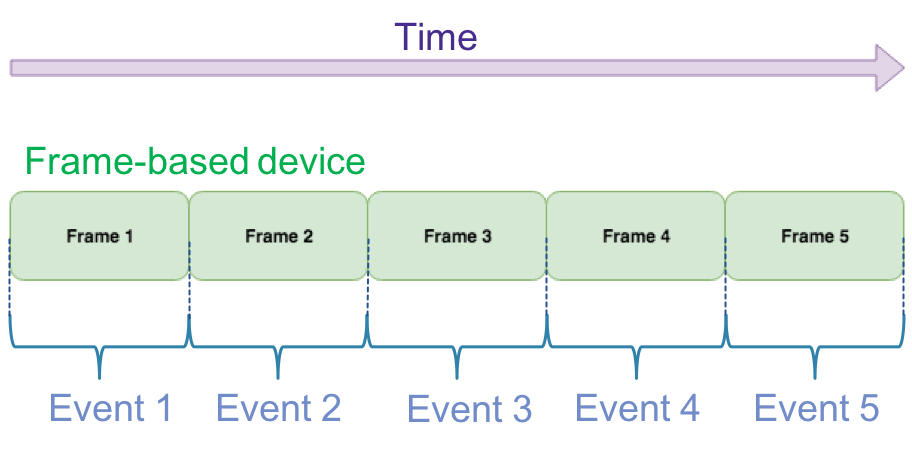
\includegraphics[width=0.66\textwidth]{framebaseddevice.png}
	\caption{text here}
	\label{fig:framebased}
\end{figure}


\begin{figure}[h]
        \centering
        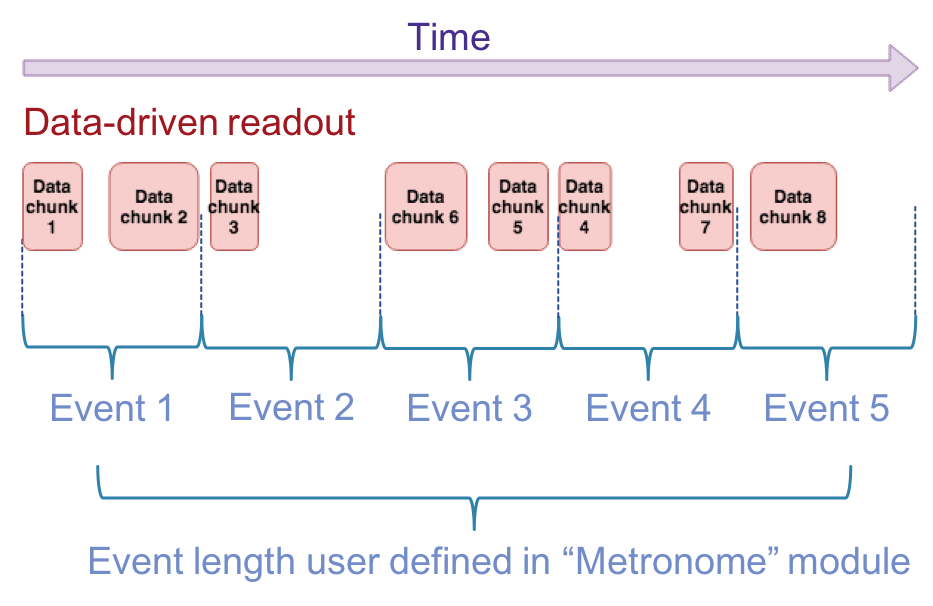
\includegraphics[width=0.66\textwidth]{datadrivendevice.png}
        \caption{text here}
        \label{fig:datadriven}
\end{figure}



\begin{figure}[h]
        \centering
        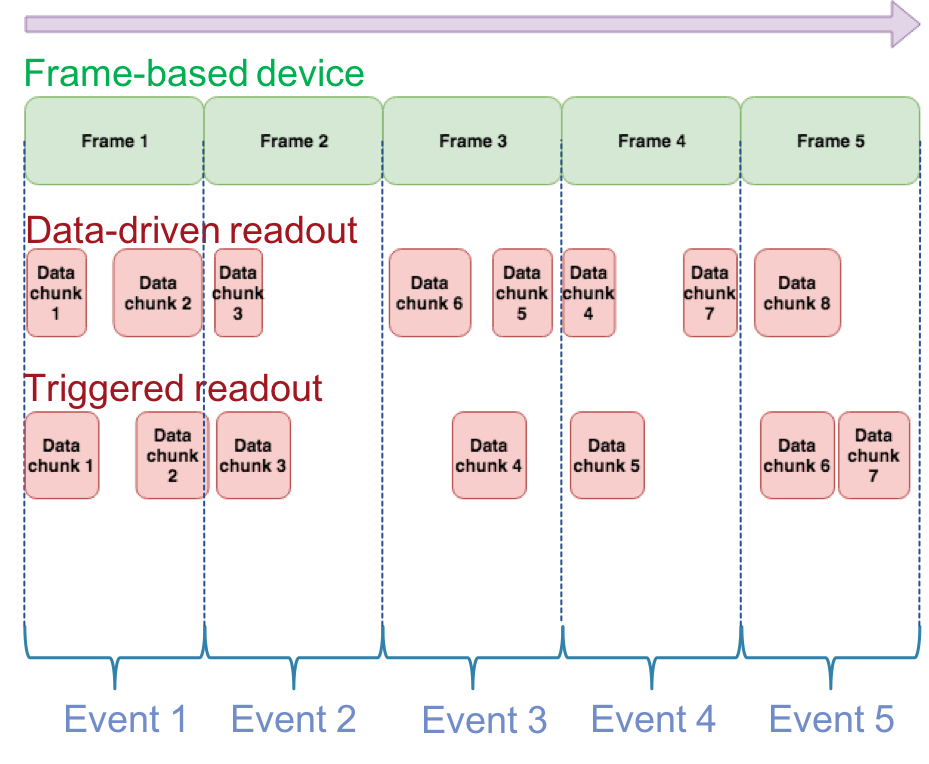
\includegraphics[width=0.66\textwidth]{datadrivenandframebased.png}
        \caption{text here}
        \label{fig:datadrivenandframebased}
\end{figure}


\chapter{Using \corry as Online Monitor}

Reconstructing test beam data with \corry does not require many dependencies and is usually very fast due to its efficient data handling and fast reconstruction routines.
It is therefore possible to directly perform a full reconstruction including tracking and analysis of the DUT data during data taking.
On Linux machines, this is even possible on the data currently recorded since multiple read pointers are allowed per file.

The \corry framework comes with an online monitoring tool in form of a module for data quality monitoring and immediate feedback to the shifter.
The \module{OnlineMonitor} is a relatively simple graphical user interface that displays and updates histograms and graphs produced by other modules during the run.
It should therefore be placed at the very end of the analysis chain in order to have access to all histograms previously registered by other modules.

\begin{figure}[tbp]
        \centering
        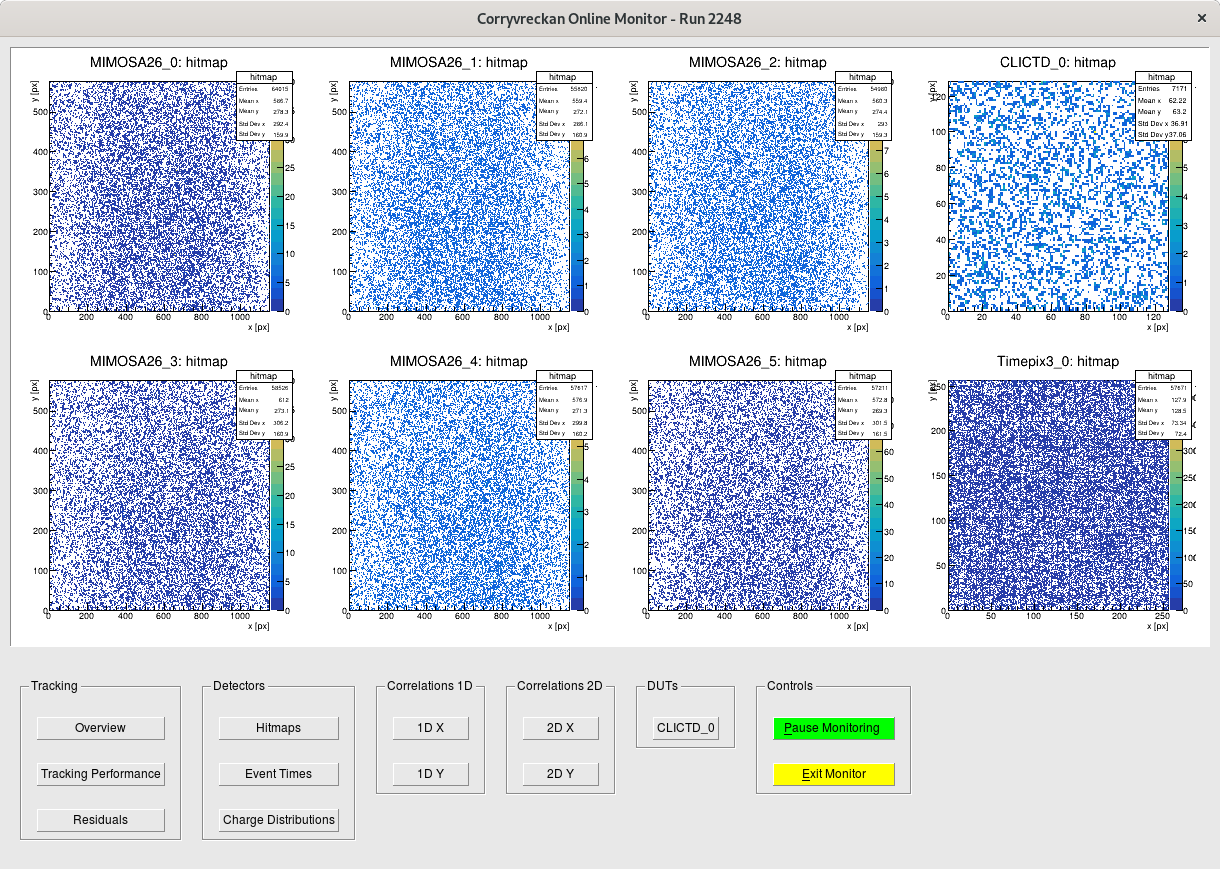
\includegraphics[width=0.9\textwidth]{onlinemon.png}
        \caption{Screenshot of the OnlineMonitor module displaying reconstruction histograms during the \corry run.}
        \label{fig:onlinemon}
\end{figure}

A screenshot of the interface is displayed in Figure~\ref{fig:onlinemon}, showing histograms from the reconstruction of data recorded with the setup presented in Section~\ref{sec:reco_mixedmode}.
The histograms are distributed over several canvases according to their stage of production in the reconstruction chain.
It is possible to display histograms for all registered detectors through the \parameter keyword in the configuration.
Histograms only from all detectors marked as DUT can be added by placing \parameter in the histogram path.

The module has a default configuration that should match many reconstruction configurations, but each of the canvases and histograms can be freely configured as described in the documentation of the \module{OnlineMonitor} in Section~\ref{onlinemonitor}.


\chapter{Alignment Procedure}
\label{ch:howtoalign}

As described in Section~\ref{sec:detector_config}, an analysis with \corry requires a configuration file defining which detectors are present in the setup.
This file also contains the position and rotation of each detector plane.
The Z-positions of all planes can \textbf{and must} be measured by hand in the existing test beam setup and entered in this configuration file for the analysis.
The X- and Y-positions as well as the rotations cannot be measured precisely by hand.
However, these have a strong influence on the tracking since a misalignment of a fraction of a millimeter might already correspond to a shift by multiple pixel pitches.

Consequently, an alignment procedure is needed in which the detector planes are shifted and rotated iteratively relative to the detector with \parameter{role = reference} to increase the tracking quality.
More technically, the track residuals on all planes,~i.e. the distribution of the spatial distance between the interpolated track intercept and the associated cluster on the plane need to be centered around zero and 'as narrow as possible' -- the width of the distribution depends on the tracking resolution of the telescope and is influenced by many factors such as the beam energy, the material budget of the detector planes, the distance between the detector planes, etc.
It is important to correctly set the \parameter{spatial_resolution} specified in the detector configuration file described in Section~\ref{sec:detector_config} because is defining the uncertainty on the cluster positions and therefore influences the track $\chi^2$.

This chapter provides a description of how to use the alignment features of \corry.
It also includes step-by-step instructions on how to align the detector planes for new set of test beam data.
Example configuration files can be found in the \dir{testing/} directory of the repository.
These are based on a Timepix3~\cite{timepix3} telescope with an ATLASpix~\cite{atlaspix} DUT at the CERN SPS with a pion beam of \SI{120}{GeV}.

For the alignment of the \textbf{reference telescope} and \textbf{device-under-test (DUT)}, the following modules are available in \corry.
\begin{itemize}
\item \module{Prealignment} for both telescope and DUT prealignment (see Section~\ref{prealignment}).
\item \module{AlignmentTrackChi2} used for telescope alignment (see Section~\ref{alignmenttrackchi2}) and is relatively robust against an initial misalignment but usually needs several iterations.
\item \module{AlignmentMillepede}, an alternative telescope alignment algorithm (see Section~\ref{alignmentmillepede}) which requires fewer iterations to reach a precise alignment but needs a better prealignment.
\item \module{AlignmentDUTResidual} used for DUT alignment (see Section~\ref{alignmentdutresidual}).
\end{itemize}

The general procedure that needs to be followed for a successful alignment is outlined here and explained in detail below.
\begin{enumerate}
\item Prealignment of the telescope (ignoring the DUT).
\item Alignment of the telescope (ignoring the DUT).
\item Prealignment of the DUT (telescope geometry is frozen).
\item Alignment of the DUT (telescope alignment is frozen).
\end{enumerate}

\begin{warning}
When using the alignment modules, the new geometry is written out to a new geometry file which needs to be specified using the parameter \parameter{detectors_file_updated}.
For details, see Section~\ref{sec:framework_parameters}.
\end{warning}

\paragraph{Correlation vs. Residual}

A spatial \textbf{correlation} plot is filled with the spatial difference of any cluster on a given detector plane minus the position of any cluster on the reference plane. No tracking is required to fill these histograms.

A spatial \textbf{residual} plot shows the difference of the interpolated track intercept onto a given plane minus the position of its associated cluster.\\

Consequently, the goal of the alignment is to force the \textbf{residuals} to be centered around zero.
The \textbf{correlations} do not necessarily have to be centered at zero as a possible offset reflects the \emph{physical displacement} of a detector plane in X and Y with respect to the reference plane.
However, it can be useful to inspect the \textbf{correlation} plots especially in the beginning when the alignment is not yet good enough for a reasonable tracking.

\section{Aligning the Telescope}
\label{sec:align_tel}
Initially, the telescope needs to be aligned.
For this, the DUT is ignored.

\subsection*{Prealignment of the Telescope}
The \module{AlignmentTrackChi2} module requires a careful prealignment. Otherwise it does not converge and the alignment will fail.
The Z-positions of all planes need to be measured by hand \textbf{in the existing test beam setup} and then adjusted in the detectors file.
For X and Y, the alignment file from an already aligned run with the same telescope plane arrangement is a solid basis to start from.
If no previous alignment is available, all values for X and Y should be set to 0.

For the prealignment, two strategies can be applied:
\begin{itemize}
\item The \module{Prealignment} module can be used (see Section~\ref{prealignment}).
\item If the above does not bring the expected result, a manual prealignment can be performed as described below.
\end{itemize}

To have a first look at the initial alignment guess, one can run
\begin{verbatim}
$ /path/to/corryvreckan/bin/corry                     \
    -c analyse_telescope.conf                         \
   [-o detectors_file=<detectorsFile>                 \
    -o histogram_file=<histogramFile>                 \
    -o EventLoaderTimepix3.input_directory=<inputDir>]
\end{verbatim}

The \parameter{spatial_cut_abs/rel} in \module{Tracking4D} should be set to multiple ($\sim4$) pixel pitch.

One can inspect the spatial correlations in X and Ythe track $\chi^2$, and the residuals with the online monitoring or by opening the generated ROOT file after finishing the script.
These can be found in the modules \module{Correlations} (see Section~\ref{correlations}) and \module{Tracking4D} (see Section~\ref{tracking4d}).

To save time, one can limit the number of processed tracks. For instance, set \parameter{number_of_events = 10000} or \parameter{number_of_tracks = 10000} (see Section~\ref{sec:framework_parameters}).

If no peak at all is apparent in the correlations or residuals, the hitmaps can be checked to see if valid data is actually available for all planes.

Now, the \texttt{[Prealignment]} module can be used.
To prealign only the telescope, the DUT can be excluded by using \parameter{type = <detector_type_of_telescope>} (e.g.~\parameter{CLICPIX2}). For details, see Section~\ref{sec:module_manager}.

To use the module, \file{align_tel.conf} needs to be edited such that \texttt{[Prealignment]} is enabled and \texttt{[Alignment]} is disabled:
\begin{minted}[frame=single,framesep=3pt,breaklines=true,tabsize=2,linenos]{ini}
...
[Prealignment]
type = <detector_type_of_telescope> # <-- optional!
[Ignore]
#[AlignmentTrackChi2]
log_level=INFO
iterations = 4
align_orientation=true
align_position=true
\end{minted}

Then one can run
\begin{verbatim}
$ /path/to/corryvreckan/bin/corry                      \
    -c align_telescope.conf                            \
   [-o detectors_file=<detectorsFile>                  \
    -o detectors_file_updated=<detectorsFileUpdated>   \
    -o histogram_file=<histogramFile>                  \
    -o EventLoaderTimepix3.input_directory=<inputDir>]
\end{verbatim}

The actual prealignment is only performed after the events have been analyzed and written to the detectors file in the finalizing step.
This means to check whether the alignment has improved, one needs to re-run the analysis or the next iteration of the alignment as the previously generated ROOT file corresponds to the initial alignment.
This is the case for every iteration of the prealignment or alignment.

Generally, it suffices to run the \texttt{[Prealignment]} module once and then proceed with the next step.

\subsubsection*{Manual Prealignment of the Telescope}
If the prealignment using the module \texttt{[Prealignment]} does not bring the expected results, one can also perform the same steps manually by investigating the residuals of the DUT with respect to tracks.
For the residuals, the shift of the peak from 0 can be estimated with a precision of $\mathcal{O}(\SI{100}{\micro m})$ by zooming in using the \texttt{TBrowser}.
For instance, if the peak is shifted by +\SI{+300}{\micro m}, the detectors file needs to be edited and \SI{+300}{\micro m} should be added to the respective position, if \SI{-300}{\micro m}, subtracted.

After modifying the positions of individual planes in the configuration file, \corry can be re-run to check the correlation and residual plots for the updated geometry.
These steps need to be iterated a few times until the peaks of the \textbf{residuals} are centered around 0.

Rotational misalignments can be inferred from the slope of the 2D spatial correlation plots, the actual rotation angle has to be calculated using the respective pixel pitches of the devices.

\begin{warning}
It is important \textbf{not} to force the peak of the spatial \textbf{correlations} to be at exactly 0 because the position of the peak corresponds to the \textit{physical displacement} of a detector plane in X and Y with respect to the reference plane.
The spatial \textbf{correlations} should \textbf{only be used} if the spatial \textbf{residual} plots are not filled reasonable due to bad tracking.
Hence, the spatial correlations can be shifted towards zero in a first iteration.
\end{warning}


\subsection*{Alignment of the Telescope}
After the prealignment, the actual \textbf{precise} alignment can be performed using the \texttt{[AlignmentTrackChi2]} module (see Section~\ref{alignmenttrackchi2}).
To this end, \file{align_tel.conf} needs to be modified such that the prealignment is disabled and the alignment is enabled:
\begin{minted}[frame=single,framesep=3pt,breaklines=true,tabsize=2,linenos]{ini}
...
#[Prealignment]
#[Ignore]
[AlignmentTrackChi2]
log_level=INFO
iterations = 4
align_orientation=true
align_position=true
\end{minted}

The algorithm performs an optimisation of the track $\chi^2$.

Typically, the alignment needs to be iterated a handful of times until the residuals (which again can be inspected in the ROOT file after re-running the analysis) are nicely centered around 0 and 'as narrow as possible' -- the RMS of the residuals corresponds to the spatial resolution of each plane (convolved with the resolution of the telescope) and should thus be $\lesssim$ pixel pitch$/\sqrt{12}$.
Starting with a \parameter{spatial_cut_abs/rel} in \texttt{[Tracking4D]} (see Section~\ref{tracking4d}) of multiple ($\sim4$) pixel pitches, it should be decreased incrementally down to the pixel pitch (e.g. run \SI{200}{\micro\m} twice, then run \SI{150}{\micro\m} twice, then \SI{100}{\micro\m} twice, and then \SI{50}{\micro\m} twice).
This allows to perform the alignment with a tight selection of very high quality tracks only.
Also the \parameter{max_track_chi2ndof} should be decreased for the same reason.
For the further analysis, the cuts can be released again.

It may happen that the procedure runs into a 'false minimum', i.e. it converges in a wrong alignment in which the residuals are clearly not centered around 0.
In this case, it is required to go one step back and improve the prealignment.

Once the alignment is done, one should obtain narrow residuals centered around 0 and a good distribution of the track $\chi^2$ as shown in Figures~\ref{fig:exampleAlignment}.
If the alignment keeps to fail, it is possible to allow only for rotational or translational alignment while freezing the other for one or a few iterations.

\begin{minted}[frame=single,framesep=3pt,breaklines=true,tabsize=2,linenos]{ini}
...
#[Prealignment]
#[Ignore]
[AlignmentTrackChi2]
log_level=INFO
iterations = 4
align_orientation=false #<-- disable rotational alignment
align_position=true
\end{minted}

\begin{figure}
    \centering
    \begin{subfigure}[t]{0.66\textwidth}
        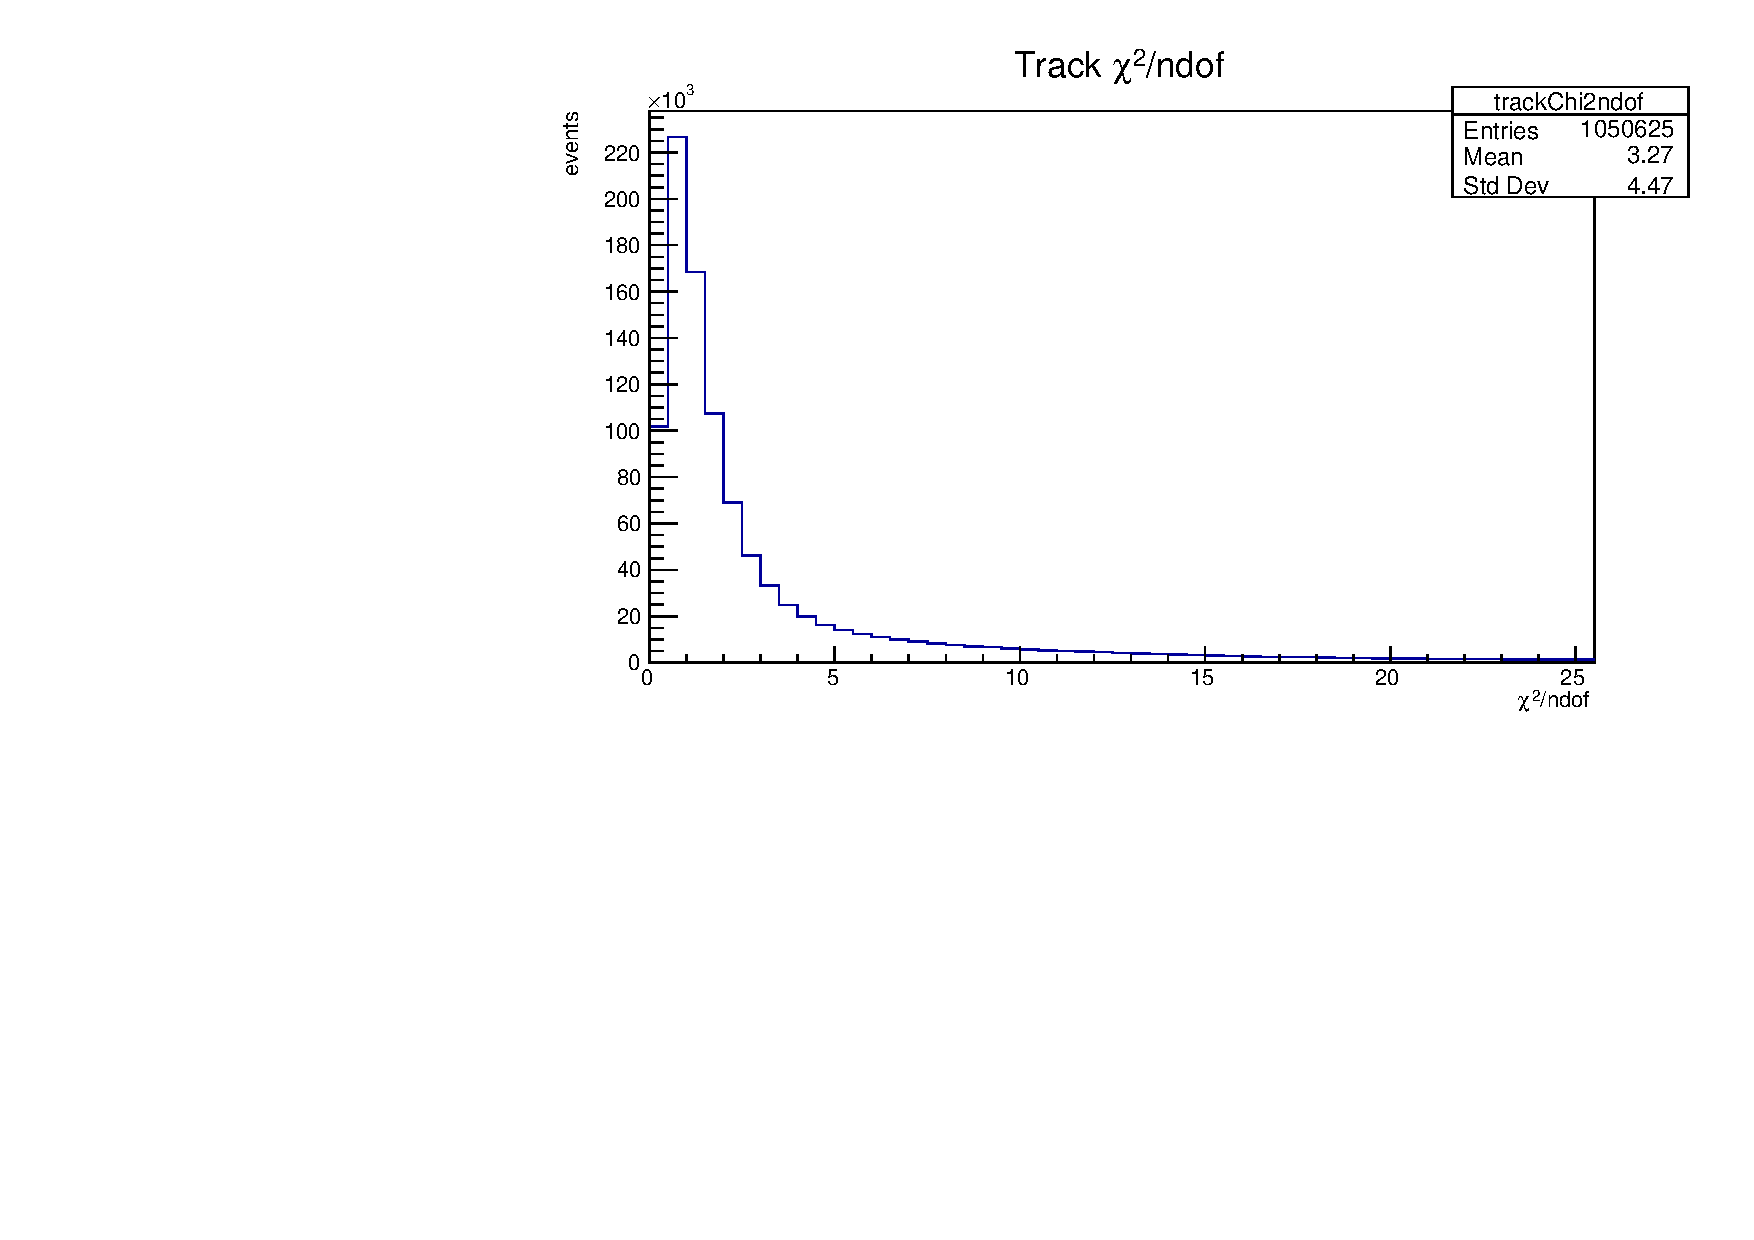
\includegraphics[width=\textwidth]{trackChi2ndof_goodexample}
        \caption{Good example of a track $\chi^2$/ndf distribution.}
        \label{fig:trackChi2}
    \end{subfigure}
    \begin{subfigure}[t]{0.66\textwidth}
        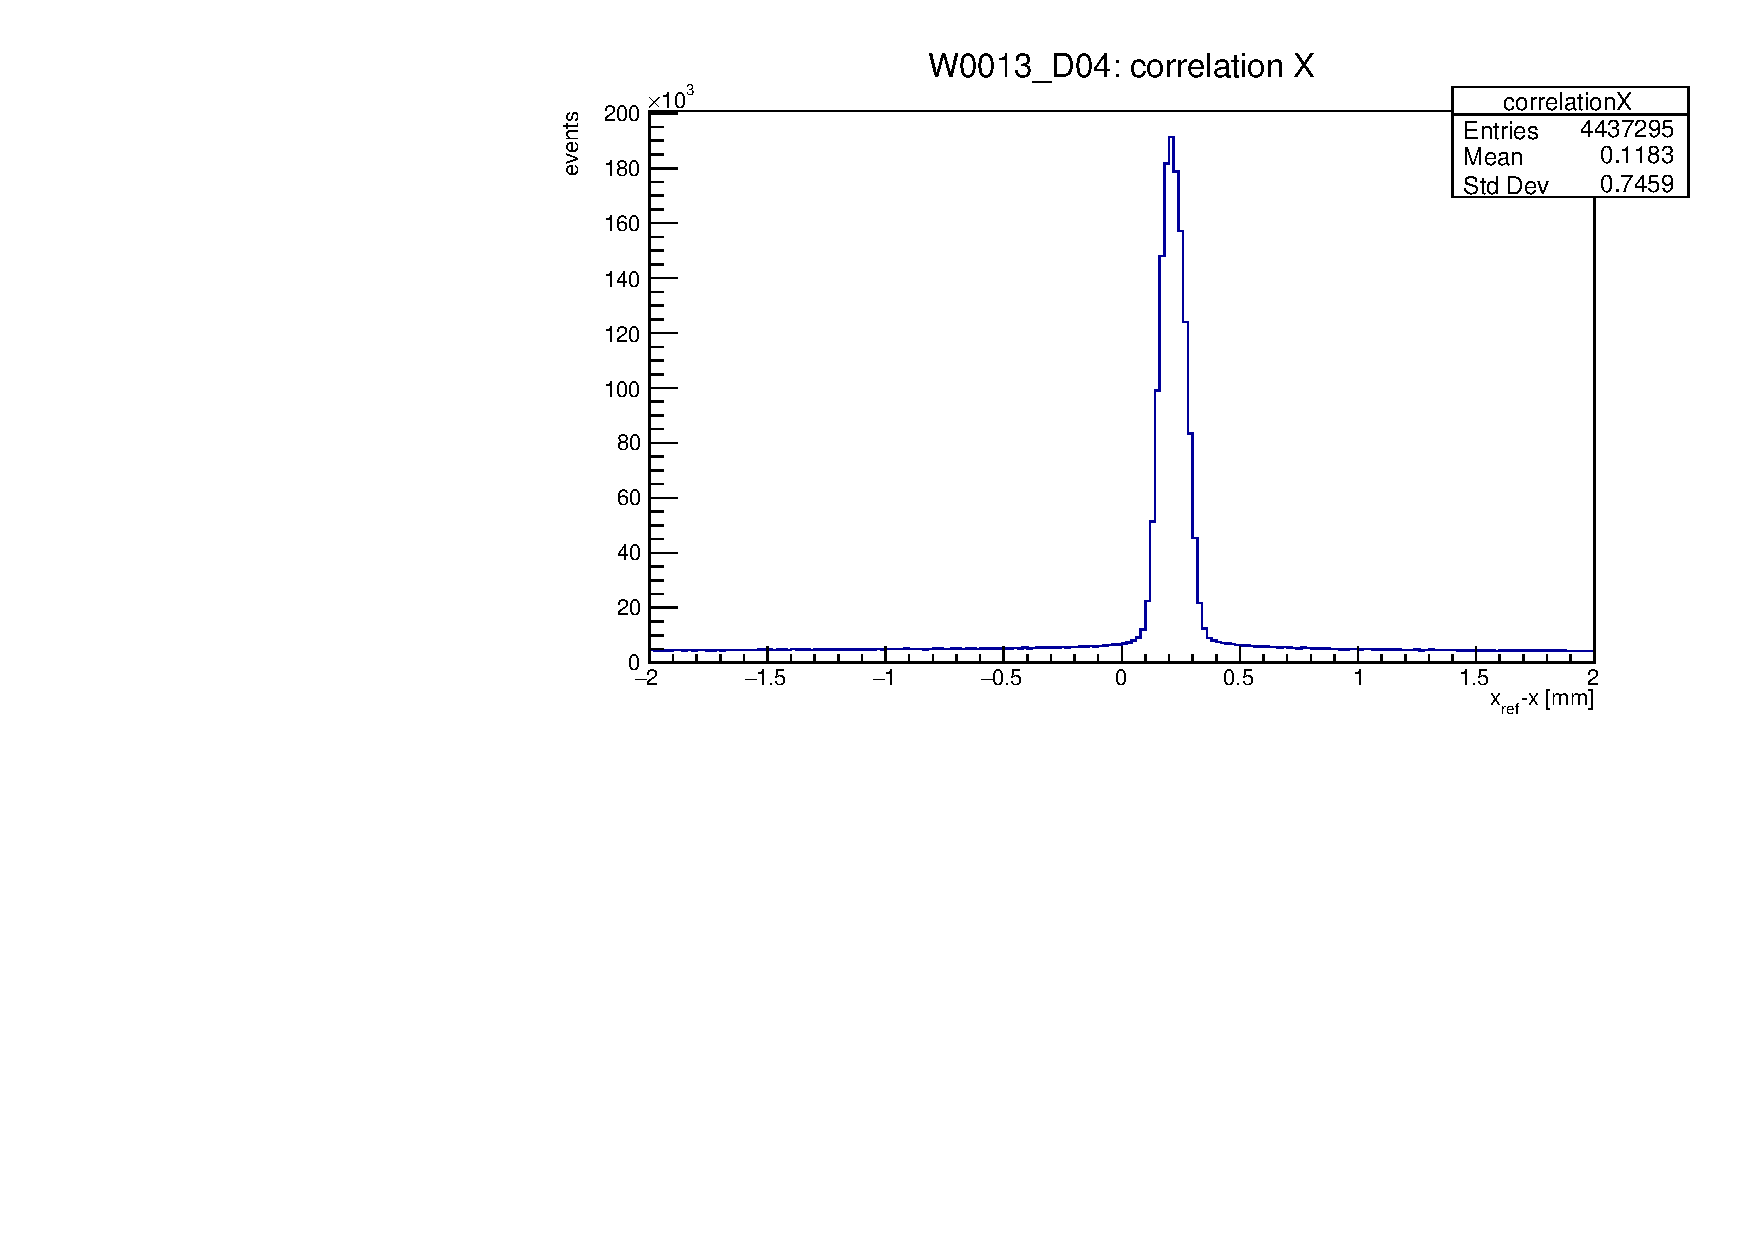
\includegraphics[width=\textwidth]{correlationX_goodexample}
        \caption{Good example of a spatial correlation plot between two telescope planes. The offset from zero corresponds to the \emph{physical displacement} of the plane  with respect to the reference plane.}
        \label{fig:correlationX}
    \end{subfigure}
    \begin{subfigure}[t]{0.66\textwidth}
        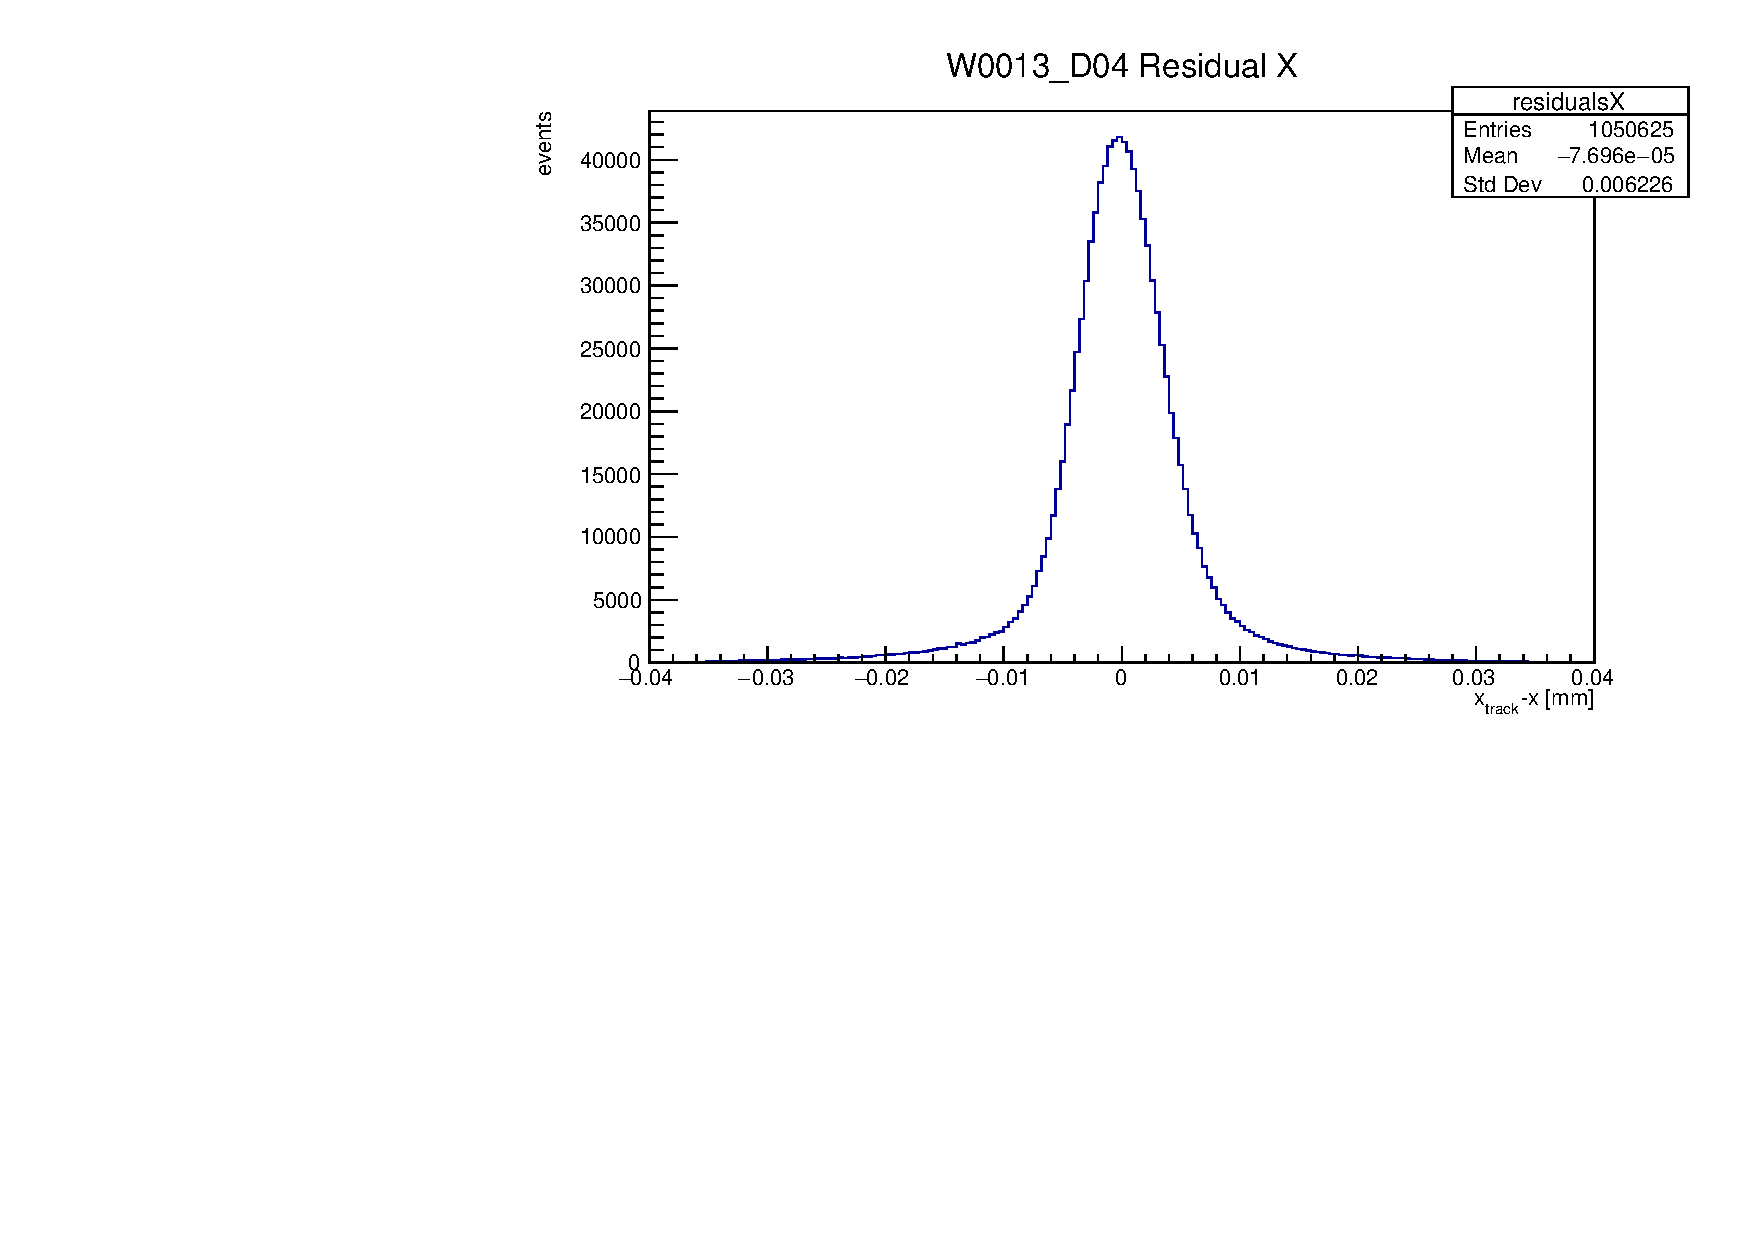
\includegraphics[width=\textwidth]{residualX_goodexample}
        \caption{Good example of a spatial residual distribution. It is centered around zero.}
        \label{fig:residualX}
    \end{subfigure}
    \caption{Examples of distributions how they should look after a successful alignment of the Timepix3 telescope at the CERN SPS with \SI{120}{\GeV} pions.}
    \label{fig:exampleAlignment}
\end{figure}

Instead of using \texttt{[AlignmentTrackChi2]}, one can also use the module \texttt{[AlignmentMillepede]} (see Section~\ref{alignmentmillepede}).
It allows a simultaneous fit of both the tracks and the alignment constants.
The modules stops if the convergence, i.e.\ the absolute sum of all corrections over the total number of parameters, is smaller than the configured value, and the alignment is complete.
It should be noted that this module requires a rather good prealignment already.

\section{Aligning the DUT}
\label{sec:align_dut}
Once the telescope is aligned, its geometry is not changed anymore. From now on, it is used to build tracks which are then matched to clusters on the DUT.

\subsection*{Prealignment of the DUT}
The prealignment of the DUT follows the same strategy as for the telescope. To look at the current alignment, the script
\begin{verbatim}
$ /path/to/corryvreckan/bin/corry                          \
    -c analyse_atlaspix.conf                               \
   [-o detectors_file=<detectorsFile>                      \
    -o histogram_file=<histogramFile>                      \
    -o EventLoaderTimepix3.input_directory=<inputDir_TPX>  \
    -o EventLoaderATLASpix.input_directory=<inputDir_APX>]
\end{verbatim}
needs to be run.
If no better guess is available, the initial alignment of the DUT should be set to $x=y=0$.

Then, by repeatedly running \corry and modifying the position of the DUT in the detectors file one should be able to bring the peaks of the spatial residuals in X and Y close to zero.
If no peak at all can be seen in the residual plots, the spatial correlations plots can be inspected. In addition, potentially parameters related to the corresponding event loader need to be corrected in the configuration file.

\begin{warning}
If using the \texttt{[Prealignment]} module, it is possible to prealign all planes at once as described above in Section~\ref{sec:align_tel}.
If only the DUT shall be prealigned here, the parameter \parameter{name = <name_of_dut>} or \parameter{type = <detector_type_of_dut>} need to be used.
Otherwise, the telescope planes are also shifted again destroying the telescope alignment.
\end{warning}

\begin{minted}[frame=single,framesep=3pt,breaklines=true,tabsize=2,linenos]{ini}
...
[Prealignment]
name = <name_of_dut> # <-- otherwise the telescope planes will be moved!

[Ignore]
#[AlignmentDUTResiduals]
log_level=INFO
iterations = 4
align_orientation=true
align_position=true
\end{minted}

\subsection*{Alignment of the DUT}
The alignment strategy for the DUT is similar as for the telescope and requires multiple iterations.
In \file{align_dut.conf}, the prealignment needs to be disabled and the alignment enabled.
Now, the algorithm optimizes the residuals of the tracks through the DUT.

\begin{minted}[frame=single,framesep=3pt,breaklines=true,tabsize=2,linenos]{ini}
...
#[Prealignment]
#[Ignore]
[AlignmentDUTResiduals]
log_level=INFO
iterations = 4
align_orientation=true
align_position=true
\end{minted}

Then run
\begin{verbatim}
$ /path/to/corryvreckan/bin/corry                          \
    -c align_dut.conf                                      \
   [-o detectors_file=<detectorsFile>                      \
    -o detectors_file_updated=<detectorsFileUpdated>       \
    -o histogram_file=<histogramFile>                      \
    -o EventLoaderTimepix3.input_directory=<inputDir_TPX>  \
    -o EventLoaderATLASpix.input_directory=<inputDir_APX>]
\end{verbatim}

Like for the telescope alignment, the RMS of the residuals can be interpreted as the spatial resolution of the DUT (convolved with the track resolution of the telescope at the position if the DUT) and should thus be $\lesssim$~pixel pitch$/\sqrt{12}$.
Again, starting with a \parameter{spatial_cut_abs/rel} in \texttt{[DUTAssociation]} (see Section~\ref{dutassociation}) of multiple ($\sim4$) pixel pitches, it should be decreased incrementally down to the pixel pitch. Note that an asymmetric pixel geometry requires the \parameter{spatial_cut_abs/rel} to be chosen accordingly.

If the alignment keeps to fail, it is possible to allow only for rotational or translational alignment while freezing the other for one or a few iterations.

\begin{minted}[frame=single,framesep=3pt,breaklines=true,tabsize=2,linenos]{ini}
...
#[Prealignment]
#[Ignore]
[AlignmentDUTResiduals]
log_level=INFO
iterations = 4
align_orientation=false #<-- disable rotational alignment
align_position=true
\end{minted}

For long runs it can occur that the DUT position changes with respect to the beam telescope, e.g. due to a missmatch of thermal expansion coefficients. For such cases it is possible to define functions describing this drift to the detector configuration file, as disussed in section~\ref{sec:alignTimeDep}. The following procedure is suggested to perform time-dependent alignment:
\begin{enumerate}
\item Run the alignment modules on a small number of events, such that statistics is sufficient for alignment but the relative drifts are negligible.
\item Process the full run without using alignment modules.
\item Check \command{residualsXVsEventTime} and \command{residualsYVsEventTime} in the \command{[AnalysisDUT]} module and fit an arbitrary function describing the profile, choosing an appropriate binning (so as not to artificially improve the residual width).
\item Pass the fitted functions to corry, as discussed in section~\ref{sec:alignTimeDep}, and re-process the run.
\end{enumerate}


% modules
This section describes the currently available Corryvreckan modules in detail.
The description comprises a description of the module implemented as well as possible configuration parameters along with their defaults.
Furthermore, a list of (potentially optional) output plots is provided.
For inquiries about certain modules or their documentation, the respective maintainers should be contacted directly.
The modules are listed in alphabetical order.

\lstset{language=Ini}
\includemodulesmd
\lstset{language=}

\chapter{Extending the \corry Framework}
\section{Writing Additional Modules}

use \command{addModule.sh} script in \dir{etc/}.

\subsection{Files of a Module}
\label{sec:module_files}
Every module directory should at minimum contain the following documents (with \texttt{ModuleName} replaced by the name of the module):
\begin{itemize}
\item \textbf{CMakeLists.txt}: The build script to load the dependencies and define the source files of the library.
\item \textbf{README.md}: Full documentation of the module.
\item \textbf{\textit{ModuleName}.h}: The header file of the module.
\item \textbf{\textit{ModuleName}.cpp}: The implementation file of the module.
\end{itemize}
These files are discussed in more detail below.
By default, all modules added to the \textit{src/modules/} directory will be built automatically by CMake.
If a module depends on additional packages which not every user may have installed, one can consider adding the following line to the top of the module's \textit{CMakeLists.txt}:
\begin{minted}[frame=single,framesep=3pt,breaklines=true,tabsize=2,linenos]{cmake}
CORRYVRECKAN_ENABLE_DEFAULT(OFF)
\end{minted}

\paragraph{CMakeLists.txt}
Contains the build description of the module with the following components:
\begin{enumerate}
\item On the first line either \parameter{CORRYVRECKAN_DETECTOR_MODULE(MODULE_NAME)}, \parameter{CORRYVRECKAN_DUT_MODULE(MODULE_NAME)} or \parameter{CORRYVRECKAN_GLOBAL_MODULE(MODULE_NAME)} depending on the type of module defined.
The internal name of the module is automatically saved in the variable \parameter{${MODULE_NAME}} which should be used as an argument to other functions.
Another name can be used by overwriting the variable content, but in the examples below, \parameter{${MODULE_NAME}} is used exclusively and is the preferred method of implementation.
For DUT and Detector modules, the type of detector this module is capable of handling can be specified by adding so-called type restrictions, e.g.\
\begin{minted}[frame=single,framesep=3pt,breaklines=true,tabsize=2,linenos]{cmake}
CORRYVRECKAN_DETECTOR_TYPE(${MODULE_NAME} "Timepix3" "CLICpix2")
\end{minted}
The module will then only be instantiated for detectors of one of the given types. This is particularly useful for event loader modules which read a very specific file format.

\item The following lines should contain the logic to load possible dependencies of the module (below is an example to load Geant4).
Only ROOT is automatically included and linked to the module.
\item A line with \texttt{\textbf{CORRYVRECKAN\_MODULE\_SOURCES(\$\{MODULE\_NAME\} \textit{sources})}} defines the module source files. Here, \texttt{sources} should be replaced by a list of all source files relevant to this module.
\item Possible lines to include additional directories and to link libraries for dependencies loaded earlier.
\item A line containing \parameter{CORRYVRECKAN_MODULE_INSTALL(${MODULE_NAME})} to set up the required target for the module to be installed to.
\end{enumerate}

A simple CMakeLists.txt for a module named \parameter{Test} which should run only on DUT detectors of type \emph{Timepix3} is provided below as an example.
\vspace{5pt}

\begin{minted}[frame=single,framesep=3pt,breaklines=true,tabsize=2,linenos]{cmake}
# Define module and save name to MODULE_NAME
CORRYVRECKAN_DUT_MODULE(MODULE_NAME)
CORRYVRECKAN_DETECTOR_TYPE(${MODULE_NAME} "Timepix3")

# Add the sources for this module
CORRYVRECKAN_MODULE_SOURCES(${MODULE_NAME}
    Test.cpp
)

# Provide standard install target
CORRYVRECKAN_MODULE_INSTALL(${MODULE_NAME})
\end{minted}

\paragraph{README.md}
The \file{README.md} serves as the documentation for the module and should be written in Markdown format~\cite{markdown}.
It is automatically converted to \LaTeX using Pandoc~\cite{pandoc} and included in the user manual in Chapter~\ref{ch:modules}.
By documenting the module functionality in Markdown, the information is also viewable with a web browser in the repository within the module sub-folder.

The \file{README.md} should follow the structure indicated in the \file{README.md} file of the \parameter{Dummy} module in \dir{src/modules/Dummy}, and should contain at least the following sections:
\begin{itemize}
\item The H1-size header with the name of the module and at least the following required elements: the \textbf{Maintainer}, the \textbf{Module Type} and the \textbf{Status} of the module.
The module type should be either \textbf{GLOBAL}, \textbf{DETECTOR}, \textbf{DUT}.
If the module is working and well-tested, the status of the module should be \textbf{Functional}.
By default, new modules are given the status \textbf{Immature}.
The maintainer should mention the full name of the module maintainer, with their email address in parentheses.
A minimal header is therefore:
\begin{verbatim}
# ModuleName
Maintainer: Example Author (<example@example.org>)
Module Type: GLOBAL
Status: Functional
\end{verbatim}
In addition, the \textbf{Detector Type} should be mentioned for modules of types \textbf{DETECTOR} and \textbf{DUT}.
\item An H3-size section named \textbf{Description}, containing a short description of the module.
\item An H3-size section named \textbf{Parameters}, with all available configuration parameters of the module.
The parameters should be briefly explained in an itemised list with the name of the parameter set as an inline code block.
\item An H3-size section named \textbf{Plots Created}, listing all plots created by this module.
\item An H3-size section with the title \textbf{Usage} which should contain at least one simple example of a valid configuration for the module.
\end{itemize}

\paragraph{\texttt{ModuleName}.h and \texttt{ModuleName}.cpp}
All modules should consist of both a header file and a source file.
In the header file, the module is defined together with all of its methods.
Brief Doxygen documentation should be added to explain what each method does.
The source file should provide the implementation of every method and also its more detailed Doxygen documentation.
Methods should only be declared in the header and defined in the source file in order to keep the interface clean.

\subsection{Module structure}
\label{sec:module_structure}
All modules must inherit from the \texttt{Module} base class, which can be found in \textit{src/core/module/Module.hpp}.
The module base class provides two base constructors, a few convenient methods and several methods which the user is required to override.
Each module should provide a constructor using the fixed set of arguments defined by the framework; this particular constructor is always called during by the module instantiation logic.
These arguments for the constructor differ for global and detector/DUT modules.

For global modules, the constructor for a \texttt{TestModule} should be:
\begin{minted}[frame=single,framesep=3pt,breaklines=true,tabsize=2,linenos]{c++}
TestModule(Configuration& config, std::vector<std::shared_ptr<Detector>> detectors): Module(std::move(config), detectors) {}
\end{minted}

For detector and DUT modules, the first argument are the same, but the last argument is a \texttt{std::shared\_ptr} to the linked detector.
It should always forward this detector to the base class together with the configuration object.
Thus, the constructor of a detector module is:
\begin{minted}[frame=single,framesep=3pt,breaklines=true,tabsize=2,linenos]{c++}
TestModule(Configuration& config, std::shared_ptr<Detector> detector): Module(std::move(config), std::move(detector)) {}
\end{minted}

In addition to the constructor, each module can override the following methods:
\begin{itemize}
\item \parameter{initialise()}: Called after loading and constructing all modules and before starting the analysis loop.
This method can for example be used to initialize histograms.
\item \parameter{run(std::shared_ptr<Clipboard> clipboard)}: Called for every time frame or triggered event to be analyzed in the simulation. The argument represents a pointer to the clipboard where the event data is stored.
A status code is returned to signal the framework whether to continue processing data or to end the run.
\item \parameter{finalise()}: Called after processing all events in the run and before destructing the module.
Typically used to save the output data (like histograms).
Any exceptions should be thrown from here instead of the destructor.
\end{itemize}


\chapter{Development Tools \& Continuous Integration}
\label{ch:testing}

The following chapter will introduce a few tools included in the framework to ease development and help to maintain a high code quality. This comprises tools for the developer to be used while coding, as well as a continuous integration (CI) and automated test cases of various framework and module functionalities.

The chapter is structured as follows.
Section~\ref{sec:targets} describes the available \command{make} targets for code quality and formatting checks, Section~\ref{sec:ci} briefly introduces the CI, and Section~\ref{sec:tests} provides an overview of the currently implemented framework, module, and performance test scenarios.

\section{Additional Targets}
\label{sec:targets}

A set of testing targets in addition to the standard compilation targets are automatically created by CMake to enable additional code quality checks and testing.
Some of these targets are used by the project's CI, others are intended for manual checks.
Currently, the following targets are provided:

\begin{description}
  \item[\command{make format}] invokes the \command{clang-format} tool to apply the project's coding style convention to all files of the code base. The format is defined in the \file{.clang-format} file in the root directory of the repository and mostly follows the suggestions defined by the standard LLVM style with minor modifications. Most notably are the consistent usage of four whitespace characters as indentation and the column limit of 125 characters.
  This can be further simplified by installing the \emph{git hook} provided in the directory \dir{/etc/git-hooks/}. A hook is a script called by \command{git} before a certain action. In this case, it is a pre-commit hook which automatically runs \command{clang-format} in the background and offers to update the formatting of the code to be committed. It can be installed by calling
  \begin{minted}[frame=single,framesep=3pt,breaklines=true,tabsize=2,linenos]{bash}
  ./etc/git-hooks/install-hooks.sh
  \end{minted}
  once.
  \item[\command{make check-format}] also invokes the \command{clang-format} tool but does not apply the required changes to the code. Instead, it returns an exit code 0 (pass) if no changes are necessary and exit code 1 (fail) if changes are to be applied. This is used by the CI.
  \item[\command{make lint}] invokes the \command{clang-tidy} tool to provide additional linting of the source code. The tool tries to detect possible errors (and thus potential bugs), dangerous constructs (such as uninitialized variables) as well as stylistic errors. In addition, it ensures proper usage of modern C++ standards. The configuration used for the \command{clang-tidy} command can be found in the \file{.clang-tidy} file in the root directory of the repository.
  \item[\command{make check-lint}] also invokes the \command{clang-tidy} tool but does not report the issues found while parsing the code. Instead, it returns an exit code 0 (pass) if no errors have been produced and exit code 1 (fail) if issues are present. This is used by the CI.
  \item[\command{make cppcheck}] runs the \command{cppcheck} command for additional static code analysis. The output is stored in the file \file{cppcheck_results.xml} in XML2.0 format. It should be noted that some of the issues reported by the tool are to be considered false positives.
  \item[\command{make cppcheck-html}] compiles a HTML report from the defects list gathered by \command{make cppcheck}. This target is only available if the \command{cppcheck-htmlreport} executable is found in the \dir{PATH}.
  \item[\command{make package}] creates a binary release tarball as described in Section~\ref{sec:packaging}.
\end{description}

\section{Packaging}
\label{sec:packaging}
\corry comes with a basic configuration to generate tarballs from the compiled binaries using the CPack command. In order to generate a working tarball from the current \corry build, the \parameter{RPATH} of the executable should not be set, otherwise the \command{corry} binary will not be able to locate the dynamic libraries. If not set, the global \parameter{LD_LIBRARY_PATH} is used to search for the required libraries:

\begin{verbatim}
$ mkdir build
$ cd build
$ cmake -DCMAKE_SKIP_RPATH=ON ..
$ make package
\end{verbatim}

The content of the produced tarball can be extracted to any location of the file system, but requires the ROOT6 and Geant4 libraries as well as possibly additional libraries linked by individual at runtime.

For this purpose, a \file{setup.sh} shell script is automatically generated and added to the tarball.
By default, it contains the ROOT6 path used for the compilation of the binaries.
Additional dependencies, either library paths or shell scripts to be sourced, can be added via CMake for individual modules using the CMake functions described below.
The paths stored correspond to the dependencies used at compile time, it might be necessary to change them manually when deploying on a different computer.

\paragraph{\texttt{\textbf{ADD\_RUNTIME\_DEP(name)}}}

This CMake command can be used to add a shell script to be sourced to the setup file.
The mandatory argument \parameter{name} can either be an absolute path to the corresponding file, or only the file name when located in a search path known to CMake, for example:

\begin{minted}[frame=single,framesep=3pt,breaklines=true,tabsize=2,linenos]{cmake}
# Add "thisroot.sh" of the ROOT framework as runtime dependency for setup.sh file:
ADD_RUNTIME_DEP(thisroot.sh)
\end{minted}

The command uses the \command{GET_FILENAME_COMPONENT} command of CMake with the \parameter{PROGRAM} option.
Duplicates are removed from the list automatically.
Each file found will be written to the setup file as

\begin{verbatim}
source <absolute path to the file>
\end{verbatim}

\paragraph{\texttt{\textbf{ADD\_RUNTIME\_LIB(names)}}}

This CMake command can be used to add additional libraries to the global search path.
The mandatory argument \parameter{names} should be the absolute path of a library or a list of paths, such as:

\begin{minted}[frame=single,framesep=3pt,breaklines=true,tabsize=2,linenos]{cmake}
# This module requires the LCIO library:
FIND_PACKAGE(LCIO REQUIRED)
# The FIND routine provides all libraries in the LCIO_LIBRARIES variable:
ADD_RUNTIME_LIB(${LCIO_LIBRARIES})
\end{minted}

The command uses the \command{GET_FILENAME_COMPONENT} command of CMake with the \parameter{DIRECTORY} option to determine the directory of the corresponding shared library.
Duplicates are removed from the list automatically.
Each directory found will be added to the global library search path by adding the following line to the setup file:

\begin{verbatim}
export LD_LIBRARY_PATH="<library directory>:$LD_LIBRARY_PATH"
\end{verbatim}

\section{Continuous Integration}
\label{sec:ci}

Quality and compatibility of the \corry framework is ensured by an elaborate continuous integration (CI) which builds and tests the software on all supported platforms.
The \corry CI uses the GitLab Continuous Integration features and consists of six distinct stages.
It is configured via the \file{.gitlab-ci.yml} file in the repository's root directory, while additional setup scripts for the GitLab CI Runner machines and the Docker instances can be found in the \dir{.gitlab-ci.d} directory.

The \textbf{compilation} stage builds the framework from the source on different platforms.
Currently, builds are performed on Scientific Linux 6, CentOS7, and Mac OS X.
On Linux type platforms, the framework is compiled with recent versions of GCC and Clang, while the latest AppleClang is used on Mac OS X.
The build is always performed with the default compiler flags enabled for the project:
\begin{verbatim}
    -pedantic -Wall -Wextra -Wcast-align -Wcast-qual -Wconversion
    -Wuseless-cast -Wctor-dtor-privacy -Wzero-as-null-pointer-constant
    -Wdisabled-optimization -Wformat=2 -Winit-self -Wlogical-op
    -Wmissing-declarations -Wmissing-include-dirs -Wnoexcept
    -Wold-style-cast -Woverloaded-virtual -Wredundant-decls
    -Wsign-conversion -Wsign-promo -Wstrict-null-sentinel
    -Wstrict-overflow=5 -Wswitch-default -Wundef -Werror -Wshadow
    -Wformat-security -Wdeprecated -fdiagnostics-color=auto
    -Wheader-hygiene
\end{verbatim}

The \textbf{testing} stage executes the framework tests described in Section~\ref{sec:tests}.
All tests are expected to pass, and no code that fails to satisfy all tests will be merged into the repository.

The \textbf{formatting} stage ensures proper formatting of the source code using the \command{clang-format} and following the coding conventions defined in the \file{.clang-format} file in the repository.
In addition, the \command{clang-tidy} tool is used for ``linting'' of the source code.
This means, the source code undergoes a static code analysis in order to identify possible sources of bugs by flagging suspicious and non-portable constructs used.
Tests are marked as failed if either of the CMake targets \command{make check-format} or \command{make check-lint} fail.
No code that fails to satisfy the coding conventions and formatting tests will be merged into the repository.

The \textbf{documentation} stage prepares this user manual as well as the Doxygen source code documentation for publication.
This also allows to identify e.g.\ failing compilation of the \LaTeX documents or additional files which accidentally have not been committed to the repository.

The \textbf{packaging} stage wraps the compiled binaries up into distributable tarballs for several platforms.
This includes adding all libraries and executables to the tarball as well as preparing the \file{setup.sh} script to prepare run-time dependencies using the information provided to the build system.
This procedure is described in more detail in Section~\ref{sec:packaging}.

Finally, the \textbf{deployment} stage is only executed for new tags in the repository.
Whenever a tag is pushed, this stages receives the build artifacts of previous stages and publishes them to the \corry project website through the EOS file system~\cite{eos}. More detailed information on deployments is provided in the following.

\section{Automatic Deployment}

The CI is configured to automatically deploy new versions of \corry and its user manual and code reference to different places to make them available to users.
This section briefly describes the different deployment end-points currently configured and in use.
The individual targets are triggered either by automatic nightly builds or by publishing new tags.
In order to prevent accidental publications, the creation of tags is protected.
Only users with \emph{Maintainer} privileges can push new tags to the repository.
For new tagged versions, all deployment targets are executed.

\subsection{Software deployment to CVMFS}
\label{sec:cvmfs}

The software is automatically deployed to CERN's VM file system (CVMFS)~\cite{cvmfs} for every new tag.
In addition, the \parameter{master} branch is built and deployed every night.
New versions are published to the folder \dir{/cvmfs/clicdp.cern.ch/software/corryvreckan/} where a new folder is created for every new tag, while updates via the \parameter{master} branch are always stored in the \dir{latest} folder.

The deployed version currently comprises all modules as well as the detector models shipped with the framework.
An additional \file{setup.sh} is placed in the root folder of the respective release, which allows to set up all runtime dependencies necessary for executing this version.
Versions both for SLC\,6 and CentOS\,7 are provided.

The deployment CI job runs on a dedicated computer with a GitLab SSH runner.
Job artifacts from the packaging stage of the CI are downloaded via their ID using the script found in \dir{.gitlab-ci.d/download_artifacts.py}, and are made available to the \emph{cvclicdp} user which has access to the CVMFS interface.
The job checks for concurrent deployments to CVMFS and then unpacks the tarball releases and publishes them to the CLICdp experiment CVMFS space, the corresponding script for the deployment can be found in \dir{.gitlab-ci.d/gitlab_deployment.sh}.
This job requires a private API token to be set as secret project variable through the GitLab interface, currently this token belongs to the service account user \emph{corry}.

\subsection{Documentation deployment to EOS}

The project documentation is deployed to the project's EOS space at \dir{/eos/project/c/corryvreckan/www/} for publication on the project website.
This comprises both the PDF and HTML versions of the user manual (subdirectory \dir{usermanual}) as well as the Doxygen code reference (subdirectory \dir{reference/}).
The documentation is only published only for new tagged versions of the framework.

The CI jobs uses the \parameter{ci-web-deployer} Docker image from the CERN GitLab CI tools to access EOS, which requires a specific file structure of the artifact.
All files in the artifact's \dir{public/} folder will be published to the \dir{www/} folder of the given project.
This job requires the secret project variables \parameter{EOS_ACCOUNT_USERNAME} and \parameter{EOS_ACCOUNT_PASSWORD} to be set via the GitLab web interface.
Currently, this uses the credentials of the service account user \emph{corry}.

\subsection{Release tarball deployment to EOS}

Binary release tarballs are deployed to EOS to serve as downloads from the website to the directory \dir{/eos/project/c/corryvreckan/www/releases}.
New tarballs are produced for every tag as well as for nightly builds of the \parameter{master} branch, which are deployed with the name \file{corryvreckan-latest-<system-tag>-opt.tar.gz}.

The files are taken from the packaging jobs and published via the \parameter{ci-web-deployer} Docker image from the CERN GitLab CI tools.
This job requires the secret project variables \parameter{EOS_ACCOUNT_USERNAME} and \parameter{EOS_ACCOUNT_PASSWORD} to be set via the GitLab web interface.
Currently, this uses the credentials of the service account user \emph{corry}.

\subsection{Building Docker images}
\label{sec:build-docker}

New \corry Docker images are automatically created and deployed by the CI for every new tag and as a nightly build from the \parameter{master} branch.
New versions are published to project Docker container registry~\cite{corry-container-registry}.
Tagged versions can be found via their respective tag name, while updates via the nightly build are always stored with the \parameter{latest} tag attached.

The final Docker image is formed from three consecutive images with different layers of software added.
The `base` image contains all build dependencies such as compilers, CMake, and git.
It derives from a CentOS7 Docker image and can be build using the \file{etc/docker/Dockerfile.base} file via the following commands:

\begin{verbatim}
# Log into the CERN GitLab Docker registry:
$ docker login gitlab-registry.cern.ch
# Compile the new image version:
$ docker build --file etc/docker/Dockerfile.base          \
               --tag gitlab-registry.cern.ch/corryvreckan/\
                     corryvreckan/corryvreckan-base     \
               .
# Upload the image to the registry:
$ docker push gitlab-registry.cern.ch/corryvreckan/\
              corryvreckan/corryvreckan-base
\end{verbatim}

The main dependency of the framework us ROOT6, which is added to the base image via the \parameter{deps} Docker image created from the file \file{etc/docker/Dockerfile.deps} via:
\begin{verbatim}
$ docker build --file etc/docker/Dockerfile.deps          \
               --tag gitlab-registry.cern.ch/corryvreckan/\
               corryvreckan/corryvreckan-deps             \
              .
$ docker push gitlab-registry.cern.ch/corryvreckan/\
              corryvreckan/corryvreckan-deps
\end{verbatim}
These images are created manually and only updated when necessary, i.e.\ if major new version of the underlying dependencies are available.

Finally, the latest revision of \corry is built using the file \file{etc/docker/Dockerfile}.
This job is performed automatically by the continuous integration and the created containers are directly uploaded to the project's Docker registry.
\begin{verbatim}
$ docker build --file etc/docker/Dockerfile                            \
               --tag gitlab-registry.cern.ch/corryvreckan/corryvreckan \
              .
\end{verbatim}

A short summary of potential use cases for Docker images is provided in Section~\ref{sec:docker}.

\section{Data-driven Functionality Tests}
\label{sec:tests}

The build system of the framework provides a set of automated tests which are executed by the CI to ensure proper functioning of the framework and its modules.
The tests can also be manually invoked from the build directory of \corry with
\begin{verbatim}
$ ctest
\end{verbatim}

Individual tests be executed or ignored using the \command{-E} (exclude) and \command{-R} (run) switches of the \command{ctest} program:
\begin{verbatim}
$ ctest -R test_timepix3tel
\end{verbatim}

The configurations of the tests can be found in the \dir{testing/} directory of the repository and are automatically discovered by CMake.
CMake automatically searches for \corry configuration files in the respective directory and passes them to the \corry executable~(cf.\ Section~\ref{sec:executable}).

Adding a new test requires placing the configuration file in the directory, specifying the pass or fail conditions based on the tags described in the following paragraph, and providing reference data as described below.

\paragraph{Pass and Fail Conditions}

The output of any test is compared to a search string in order to determine whether it passed or failed.
These expressions are simply placed in the configuration file of the corresponding tests, a tag at the beginning of the line indicates whether it should be used for passing or failing the test.
Each test can only contain one passing and one failing expression.
If different functionality and thus outputs need to be tested, a second test should be added to cover the corresponding expression.

\begin{description}
  \item[Passing a test] The expression marked with the tag \parameter{#PASS} has to be found in the output in order for the test to pass. If the expression is not found, the test fails.
  \item[Failing a test] If the expression tagged with \parameter{#FAIL} is found in the output, the test fails. If the expression is not found, the test passes.
  \item[Depending on another test] The tag \parameter{#DEPENDS} can be used to indicate dependencies between tests, e.g.\ if a test requires a data file produced by another test.
  \item[Defining a timeout] For performance tests the runtime of the application is monitored, and the test fails if it exceeds the number of seconds defined using the \parameter{#TIMEOUT} tag.
  \item[Adding additional CLI options] Additional module command line options can be specified for the \parameter{corry} executable using the \parameter{#OPTION} tag, following the format found in Section~\ref{sec:executable}. Multiple options can be supplied by repeating the \parameter{#OPTION} tag in the configuration file, only one option per tag is allowed.
  \item[Providing datasets] The \parameter{#DATASET} tag allows to specify a configured data set which has to be available in order for the test to be executed. Datasets and their configuration is described below. Only one data set per tag is allowed, multiple tags can be used.
\end{description}

\paragraph{Providing Reference Datasets}

Reference datasets for testing are centrally stored on EOS at \dir{/eos/project/c/corryvreckan/www/data/} and are accessible over the internet. The \file{download_data.py} tool provided in the \dir{testing/} directory of the framework is capable of downloading individual data files, checking their integrity via an SHA256 hash and decompressing the tar archives.

Each test can specify one or several data sets it requires to be present in order to successfully run via the \parameter{#DATASET} tag in the configuration file. The datasets have to be made known to the download script together with their calculated SHA256 hashes when adding a new test to the repository. The file name and hash have to be added to the Python \parameter{DATASETS} array, and the file of the dataset has to be uploaded manually to EOS by one of the framework maintainers. The SHA256 hash can be generated by executing:
\begin{verbatim}
openssl sha256 <dataset>
\end{verbatim}

Paths in the test configuration files should be provided relative to the \dir{testing/} directory, all downloaded data will be stored in individual subdirectories per dataset following the naming scheme \dir{testing/data/<dataset>}.


% additional tools and resources
\section{Additional Tools \& Resources}
\label{sec:additional_tools_resources}

The following section briefly describes tools provided with the Corryvreckan framework.

\inputmd{jobsub.tex}
% FIXME This label is not required to bind correctly
\label{sec:jobsub}

\clearpage

\appendix

\clearpage
\phantomsection
\addreferencesline
\printbibliography

\end{document}
